\documentclass[11pt]{article}
\usepackage[margin=1in]{geometry}
\usepackage{amsmath,amssymb,amsthm,graphicx,booktabs,multirow,threeparttable,setspace,array}
\usepackage[round]{natbib}
\usepackage[hidelinks]{hyperref}
\usepackage{caption,enumitem,tikz,pgfplots}
\usetikzlibrary{positioning}
\pgfplotsset{compat=1.17}
\definecolor{npblue}{RGB}{31,78,121}
\definecolor{npmid}{RGB}{72,120,168}
\definecolor{gred}{RGB}{176,74,74}
\definecolor{gold}{RGB}{200,162,74}
\captionsetup{font=small,labelfont=bf}
\setstretch{1.3}
\newcommand{\VaR}{\mathrm{VaR}}
\newcommand{\ES}{\mathrm{ES}}
\newtheorem{proposition}{Proposition}
\newtheorem{lemma}{Lemma}
\renewcommand{\thefigure}{OA.\arabic{figure}}
\renewcommand{\thetable}{OA.\arabic{table}}
\renewcommand{\thesection}{OA.\arabic{section}}
\title{Online Appendix\\ \large When Do Flexible Tail-Risk Models Beat GARCH? Post-Shock Scale Error, Residual Shape, and a Real-Time Score}
\author{Sean Qin}
\date{September 2026}
\begin{document}
\maketitle
\section{Glossary of acronyms}
\begin{tabular}{@{}lp{0.8\textwidth}@{}}
\toprule
ARCD & autoregressive conditional density model \citep{hansen1994ARCD} \\
CAViaR & conditional autoregressive value-at-risk \citep{engle2004caviar}; SAV, its symmetric absolute value form \\
CC, UC & conditional coverage \citep{christoffersen1998} and unconditional coverage \citep{kupiec1995} exception tests \\
CRPS & continuous ranked probability score \\
CRSP, WRDS & Center for Research in Security Prices; Wharton Research Data Services \\
DM & Diebold--Mariano test \citep{dieboldmariano1995} \\
EM, IG, OAS & emerging markets; investment grade; option-adjusted spread \\
ERM & empirical risk minimization \\
ES, VaR & Expected Shortfall; Value-at-Risk \\
EVT, GPD & extreme-value theory; generalized Pareto distribution \\
EWMA & exponentially weighted moving average variance \citep{riskmetrics1996} \\
FHS, HS & filtered historical simulation \citep{baroneadesi1999fhs}; historical simulation \\
FRTB & Fundamental Review of the Trading Book \citep{bcbs2019frtb} \\
FWER & family-wise error rate \\
FZ0 & the zero-homogeneous Fissler--Ziegel joint (VaR, ES) scoring function \citep{fissler2016, patton2019} \\
GARCH, GJR & generalized autoregressive conditional heteroskedasticity \citep{bollerslev1986}; the Glosten--Jagannathan--Runkle leverage form \citep{glosten1993} \\
GAS & generalized autoregressive score model \citep{patton2019} \\
GBC & generative Bayesian computation \citep{polson2023gbc} \\
GBM & gradient boosting machine (gradient-boosted regression trees) \\
GFC & the 2008 global financial crisis \\
IQN & implicit quantile network \citep{dabney2018iqn} \\
MCS & Model Confidence Set \citep{hansen2011mcs} \\
PIT & probability integral transform \\
PZC & Patton, Ziegel and Chen \citep{patton2019} \\
QML & quasi-maximum likelihood \\
RV & realized variance \\
SPA & superior predictive ability test \citep{hansen2005spa} \\
TAQ & NYSE Trade and Quote database \\
\bottomrule
\end{tabular}

\section{Algorithms}
\medskip\noindent\fbox{\parbox{0.96\textwidth}{
\textbf{Algorithm OA.1 (amortized shape model).}
(i)~Assemble the pooled panel $\{(s_{j,t}, \widehat{z}_{j,t})\}$ over
names $j$ and days $t$.
(ii)~Train $H_\phi$ by SGD on
$\mathbb{E}_{\tau\sim\lambda}\,\rho_\tau(\widehat{z} - H_\phi(s,\tau))$
[network], or boost per-$\tau$ regressions on a grid [trees]; enforce
monotonicity by rearrangement.
(iii)~For any asset, including one with no return history, using characteristics-only $s$, evaluate $H_\phi(s_t,\cdot)$; no per-asset
estimation step exists.
(iv)~To \emph{sample}, draw $\tau^{(m)}\sim U(0,1)$ and return
$z^{(m)} = H_\phi(s_t,\tau^{(m)})$.
}}

\medskip\noindent\fbox{\parbox{0.96\textwidth}{
\textbf{Algorithm OA.2 (the misspecification meter, as deployed).}
(i)~Fit equation~(2) of the paper on a trailing window; store
$\widehat{z}_{t-62},\dots,\widehat{z}_t$.
(ii)~Compute $\mathrm{mk}_{63}$, $|\mathrm{sk}_{63}|$, $J_5$ by
equation~(6) of the paper.
(iii)~Convert each to its percentile against the trailing pooled panel
(same asset class); the score is the maximum of the three percentiles,
re-ranked into deciles.
(iv)~Act by the paper: top decile $\Rightarrow$ the parametric
model's average pinball loss runs $\sim$2--3\% higher within this
score region (a conditional average, not a per-name point estimate), flag the asset for the nonparametric /
residual-hybrid engine and for model-risk review; elsewhere
$\Rightarrow$ no action (in the amortized setting the engine is run
regardless; the meter serves surveillance, and day-level switching is
unsupported, Section~4.3 of the paper).
(v)~Latency: detection lags episode onset by median 0 / mean 2--4 days;
the edge is back-loaded within episodes, so the lag forfeits little.
}}

\medskip\noindent\textbf{Deployed pipeline.} Each day: (i)~update each name's GARCH filter state
$\widehat\sigma_{t+1}$ (recursion only; parameters refit annually);
(ii)~assemble the state vector $s_t$ and evaluate the shared shape model $q_\phi(\tau\mid s_t)$, one model for the whole book, no
per-name estimation; (iii)~apply the frozen GPD tail below $p_0$
and, where the desk elects the coverage overlay, the adaptive conformal shift
$c_\tau$, updated from the previous day's panel breach frequency; (iv)~report
$\widehat Q_{t+1}(\tau) = \widehat\mu+\widehat\sigma_{t+1}\,\big(Q^{z}_{t+1}(\tau)+c_\tau\big)$
at the desk's levels, with VaR and ES$_{97.5}$ both read from the coherent
min-envelope curve $Q^{z}$ of equation~(5) of the paper (VaR at the $\alpha$
node, ES its numerical tail integral); (v)~read
the misspecification score equation~(6) of the paper as the model-risk monitor: top decile means the parametric fallback's conditional average loss
in that score region runs $\sim$2--3\% higher. \emph{Annually:} refit filters, retrain the shape model,
re-estimate the tail, all on trailing data. \emph{New listing:}
run a pooled peer proxy or the characteristics-only amortized forecaster (the proxy is the more accurate in the first weeks; Section~6 of the paper) until an
own-history sample sufficient to initialize the per-name scale filter
accrues; then attach this residual-hybrid pipeline. Total marginal
cost per name per day: one filter update and
one model evaluation.

\section{Supplementary figures}
% order fixes numbering: OA.1 timing, OA.2 passrates, OA.3 horizon, OA.4 frtb, OA.5 universes, OA.6 frontier
\begin{figure}[htbp]
\centering
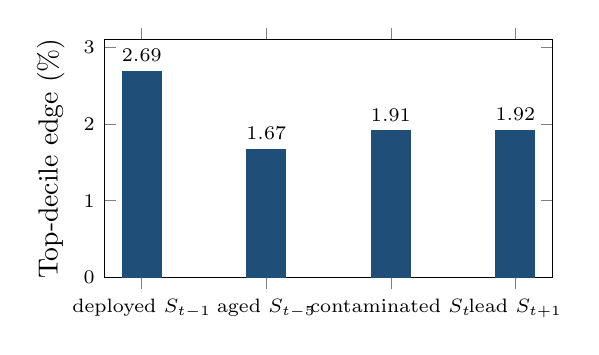
\begin{tikzpicture}
\begin{axis}[width=0.6\textwidth, height=4.6cm, ybar, bar width=14pt,
  symbolic x coords={deployed $S_{t-1}$, aged $S_{t-5}$, contaminated $S_t$, lead $S_{t+1}$},
  xtick=data, ymin=0, ymax=3.1, ylabel={Top-decile edge (\%)},
  x tick label style={font=\scriptsize}, tick label style={font=\scriptsize},
  nodes near coords, every node near coord/.append style={font=\scriptsize}]
\addplot[fill=npblue, draw=npblue] coordinates
  {(deployed $S_{t-1}$,2.69) (aged $S_{t-5}$,1.67) (contaminated $S_t$,1.91) (lead $S_{t+1}$,1.92)};
\end{axis}
\end{tikzpicture}
\caption{Timing diagnostics for the frontier. Top-decile edge under four
alignments of the mk$_{63}$ score with the daily loss (200 CRSP names;
per-date DM 5.5--6.5 in all four). The deployed lag dominates, and the
contaminated same-day alignment yields less, the opposite of what a look-ahead artifact would produce.}
\label{fig:timing}
\end{figure}
\clearpage
\begin{figure}[htbp]
\centering
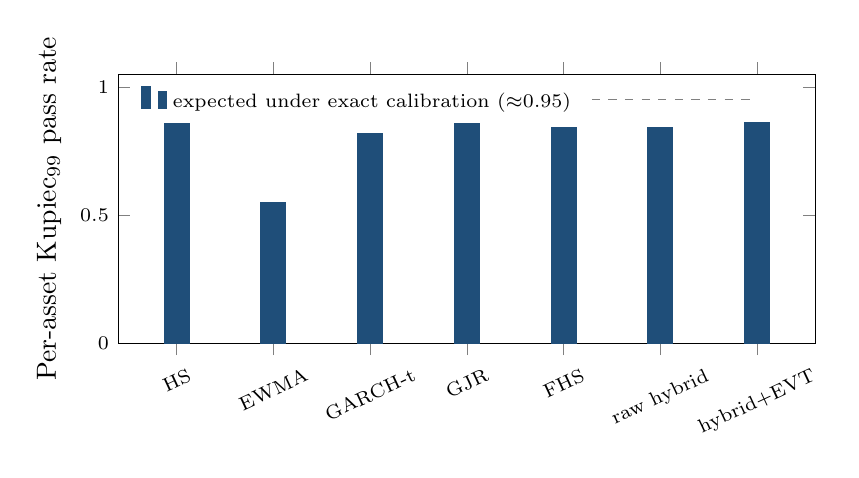
\begin{tikzpicture}
\begin{axis}[width=0.86\textwidth, height=5cm, ybar, bar width=9pt,
  symbolic x coords={HS, EWMA, GARCH-t, GJR, FHS, raw hybrid, hybrid+EVT},
  xtick=data, ymin=0, ymax=1.05, ylabel={Per-asset Kupiec$_{99}$ pass rate},
  x tick label style={font=\scriptsize, rotate=25}, tick label style={font=\scriptsize},
  legend style={font=\scriptsize, at={(0.02,0.98)}, anchor=north west, draw=none}]
\addplot[fill=npblue, draw=npblue] coordinates
  {(HS,0.93) (EWMA,0.55) (GARCH-t,0.82) (GJR,0.88) (FHS,0.84) (raw hybrid,0.84) (hybrid+EVT,0.86)};
\addplot[dashed, sharp plot, gray, mark=none] coordinates {(HS,0.95) (hybrid+EVT,0.95)};
\addlegendentry{expected under exact calibration ($\approx$0.95)}
\end{axis}
\end{tikzpicture}
\caption{Exception tests restated per asset (200 CRSP names, 99\% VaR, the rows of Table~4 of the paper):
share of names whose individual Kupiec test is consistent with nominal.
HS over-covers (conservative); EWMA fails; the EVT-tailed engine matches
the parametric benchmarks while beating them on loss and the joint
FZ0 score
(Table~4 of the paper). Date-clustered tests in the table notes.}
\label{fig:passrates}
\end{figure}
\clearpage
\begin{figure}[htbp]
\centering
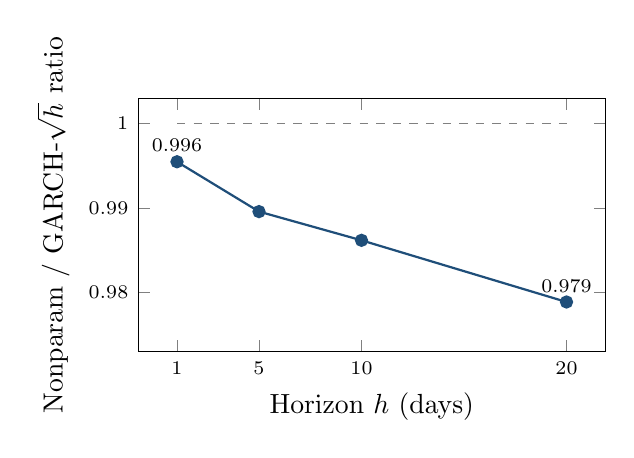
\begin{tikzpicture}
\begin{axis}[width=0.62\textwidth, height=4.8cm,
  xlabel={Horizon $h$ (days)}, ylabel={Nonparam / GARCH-$\sqrt{h}$ ratio},
  xtick={1,5,10,20}, ymin=0.973, ymax=1.003,
  tick label style={font=\scriptsize}]
\addplot[color=npblue, mark=*, thick] coordinates
  {(1,0.9955) (5,0.9896) (10,0.9862) (20,0.9789)};
\addplot[dashed, gray, mark=none] coordinates {(1,1) (20,1)};
\node[font=\scriptsize, anchor=south] at (axis cs:20,0.9789) {0.979};
\node[font=\scriptsize, anchor=south] at (axis cs:1,0.9955) {0.996};
\end{axis}
\end{tikzpicture}
\caption{The edge grows with horizon. Direct-model/GARCH pinball
ratio at $h = 1, 5, 10, 20$ days (150-name design panel; training
labels whose $h$-day window crosses the split are purged): the
$\sqrt{h}$ rule holds the one-day variance flat across the window while
the fitted GARCH variance mean-reverts, and the gap grows with the
horizon, from $0.45\%$ at $h{=}1$ to $2.1\%$ at $h{=}20$; at $h{=}10$ an
iterated-variance GARCH-$t$ benchmark removes about half of it (main text,
ten-day subsection). The forecaster is the
direct multi-day model of the main text's ten-day subsection,
\emph{not} the residual-hybrid engine, whose architecture is
one-day.}
\label{fig:horizon}
\end{figure}
\clearpage
\begin{figure}[htbp]
\centering
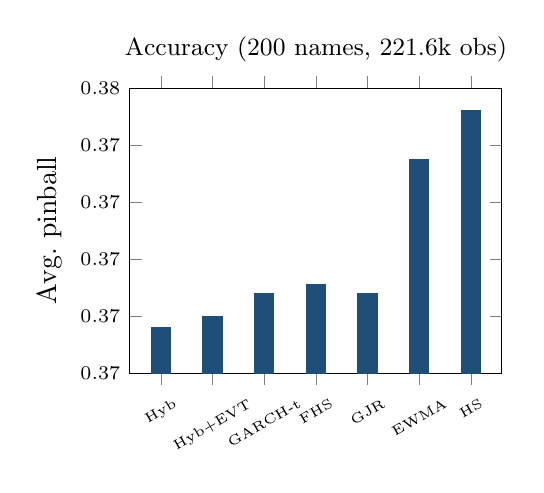
\begin{tikzpicture}
\begin{axis}[width=0.52\textwidth, height=5.2cm, ybar, bar width=7pt,
  symbolic x coords={Hyb, Hyb+EVT, GARCH-t, FHS, GJR, EWMA, HS},
  xtick=data, ymin=0.366, ymax=0.376,
  ylabel={Avg.\ pinball}, x tick label style={font=\tiny, rotate=30},
  tick label style={font=\scriptsize},
  title={\small Accuracy (200 names, 221.6k obs)}]
\addplot[fill=npblue, draw=npblue] coordinates
  {(Hyb,0.3676) (Hyb+EVT,0.3680) (GARCH-t,0.3688) (FHS,0.3691)
   (GJR,0.3688) (EWMA,0.3735) (HS,0.3752)};
\end{axis}
\end{tikzpicture}\hfill
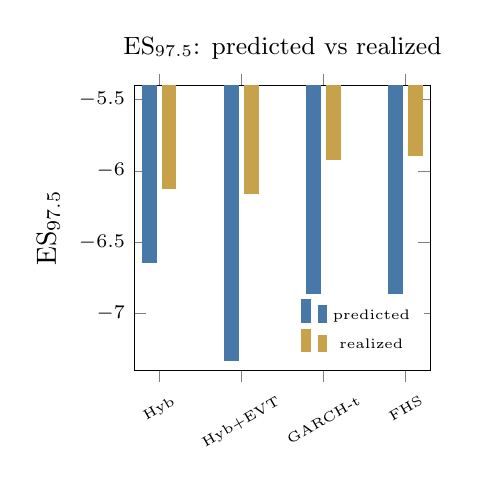
\begin{tikzpicture}
\begin{axis}[width=0.44\textwidth, height=5.2cm, ybar, bar width=5pt,
  symbolic x coords={Hyb, Hyb+EVT, GARCH-t, FHS},
  xtick=data, ymin=-7.4, ymax=-5.4,
  ylabel={ES$_{97.5}$}, x tick label style={font=\tiny, rotate=30},
  tick label style={font=\scriptsize},
  title={\small ES$_{97.5}$: predicted vs realized},
  legend style={font=\tiny, at={(0.98,0.02)}, anchor=south east,
                draw=none}]
\addplot[fill=npmid, draw=npmid] coordinates
  {(Hyb,-6.64) (Hyb+EVT,-7.33) (GARCH-t,-6.98) (FHS,-7.17)};
\addlegendentry{predicted}
\addplot[fill=gold, draw=gold] coordinates
  {(Hyb,-6.12) (Hyb+EVT,-6.16) (GARCH-t,-5.92) (FHS,-5.89)};
\addlegendentry{realized}
\end{axis}
\end{tikzpicture}
\caption{The FRTB battery. Left: average pinball loss by model (axis
truncated to resolve the ordering; differences carry DM 5.6--9.6 vs the
hybrid, all $p \approx 0$); CAViaR, not shown, statistically ties the
hybrid. Right: ES$_{97.5}$ predicted (the tail integral of Table~4 of the paper) vs realized
below each model's own VaR, a model-dependent diagnostic, not a
ranking (every fat-tailed entrant's integral exceeds its own-tail
mean); the joint FZ0 score of the paper is the ranking criterion.}
\label{fig:frtb}
\end{figure}
\clearpage
\begin{figure}[htbp]
\centering
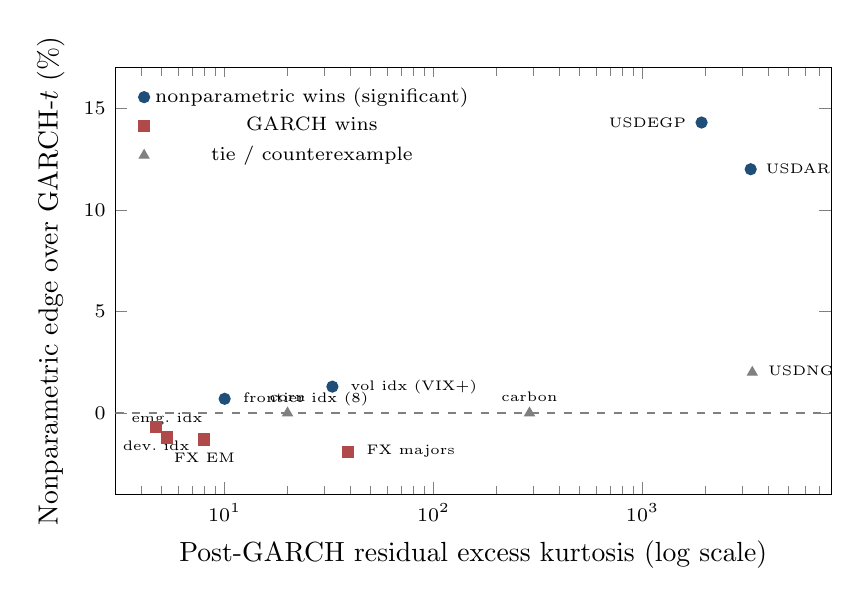
\begin{tikzpicture}
\begin{axis}[width=0.88\textwidth, height=7cm, xmode=log,
  xlabel={Post-GARCH residual excess kurtosis (log scale)},
  ylabel={Nonparametric edge over GARCH-$t$ (\%)},
  ymin=-4, ymax=17, xmin=3, xmax=8000,
  tick label style={font=\scriptsize},
  legend style={font=\scriptsize, at={(0.02,0.98)}, anchor=north west,
                draw=none}]
\addplot[only marks, mark=*, color=npblue] coordinates
  {(10,0.7) (32.8,1.3) (1920,14.3) (3298,12.0)};
\addlegendentry{nonparametric wins (significant)}
\addplot[only marks, mark=square*, color=gred] coordinates
  {(4.7,-0.7) (5.3,-1.2) (8,-1.3) (39,-1.9)};
\addlegendentry{GARCH wins}
\addplot[only marks, mark=triangle*, color=gray] coordinates
  {(20,0) (288,0) (3357,2.0)};
\addlegendentry{tie / counterexample}
\node[font=\tiny, anchor=west] at (axis cs:11,0.7) {frontier idx (8)};
\node[font=\tiny, anchor=west] at (axis cs:36,1.3) {vol idx (VIX+)};
\node[font=\tiny, anchor=east] at (axis cs:1800,14.3) {USDEGP};
\node[font=\tiny, anchor=west] at (axis cs:3500,12.0) {USDARS};
\node[font=\tiny, anchor=north] at (axis cs:4.7,-0.9) {dev.\ idx};
\node[font=\tiny, anchor=south] at (axis cs:5.3,-1.1) {emg.\ idx};
\node[font=\tiny, anchor=north] at (axis cs:8,-1.5) {FX EM};
\node[font=\tiny, anchor=west] at (axis cs:43,-1.9) {FX majors};
\node[font=\tiny, anchor=south] at (axis cs:20,0.1) {corn};
\node[font=\tiny, anchor=south] at (axis cs:288,0.1) {carbon};
\node[font=\tiny, anchor=west] at (axis cs:3600,2.0) {USDNGN (ns)};
\draw[dashed, gray] (axis cs:3,0) -- (axis cs:8000,0);
\end{axis}
\end{tikzpicture}
\caption{The frontier across universes: nonparametric edge vs post-GARCH
residual kurtosis, tier means and single assets with study-reported
kurtosis only (country universe corr 0.53; cross-asset corr 0.43).
The hyperinflation-FX tier (kurtosis $\sim$2000--3300) carries the only
decisive standalone wins; high kurtosis is predictive but neither necessary nor sufficient: carbon (288) and corn (20) tie, and NGN's win is not significant.
The Korea-2026 crash (kurtosis 4--13, GARCH wins all 23 assets, one correlated event examined after the fact, so illustrative) sits
in the lower-left regime.}
\label{fig:universes}
\end{figure}
\clearpage
\begin{figure}[htbp]
\centering
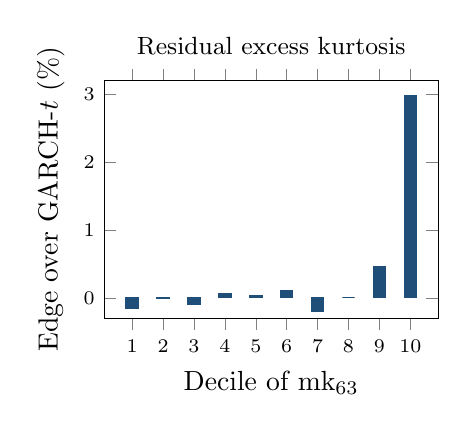
\begin{tikzpicture}
\begin{axis}[width=0.48\textwidth, height=4.6cm, ybar, bar width=4.5pt,
  xlabel={Decile of $\mathrm{mk}_{63}$}, ylabel={Edge over GARCH-$t$ (\%)},
  xtick={1,2,3,4,5,6,7,8,9,10}, ymin=-0.3, ymax=3.2,
  title={\small Residual excess kurtosis}, tick label style={font=\scriptsize}]
\addplot[fill=npblue, draw=npblue] coordinates
  {(1,-0.16)(2,-0.01)(3,-0.10)(4,0.07)(5,0.03)(6,0.11)(7,-0.20)(8,0.00)(9,0.46)(10,2.98)};
\end{axis}
\end{tikzpicture}\hfill
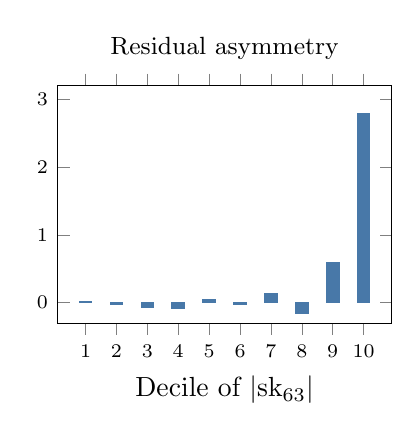
\begin{tikzpicture}
\begin{axis}[width=0.48\textwidth, height=4.6cm, ybar, bar width=4.5pt,
  xlabel={Decile of $|\mathrm{sk}_{63}|$},
  xtick={1,2,3,4,5,6,7,8,9,10}, ymin=-0.3, ymax=3.2,
  title={\small Residual asymmetry}, tick label style={font=\scriptsize}]
\addplot[fill=npmid, draw=npmid] coordinates
  {(1,0.01)(2,-0.03)(3,-0.07)(4,-0.08)(5,0.04)(6,-0.03)(7,0.14)(8,-0.16)(9,0.59)(10,2.78)};
\end{axis}
\end{tikzpicture}
\caption{The misspecification frontier. Nonparametric pinball edge over
GARCH-$t$ by decile of the trailing 63-day residual excess kurtosis
(left) and residual asymmetry (right), 200 CRSP names, 221.6k test
asset-days. Deciles 1--8 lie within $\pm0.2\%$ (values from
\texttt{composite\_profiles\_results.json}); the edge jumps in the top decile
($+2.98\%$ kurtosis, $+2.78\%$ asymmetry; per-date DM 10.5 in the top
kurtosis decile).}
\label{fig:frontier}
\end{figure}
\clearpage
\section{Supplementary tables}
\begin{table}[htbp]
\centering\small
\begin{threeparttable}
\caption{Summary of the paper's results and scope conditions. Edges are
percentage pinball reductions unless noted; DM statistics are per-date
(conventions note of Section~3 of the paper), one-sided. Panel A: the main results, each
attached to the configuration of Table~1 of the paper that carries it (no detectable loss in any
region; calm-cell 90\% lower confidence bounds sit above $-0.25\%$). A separate block reports the
direct multi-day extension, which is not the estimator. Panel B: boundary
evidence from configurations not deployed, which motivates the design.}
\label{tab:winloss}
\footnotesize\setlength{\tabcolsep}{3.5pt}
\begin{tabular}{>{\raggedright\arraybackslash}p{0.34\textwidth}>{\raggedright\arraybackslash}p{0.20\textwidth}>{\raggedright\arraybackslash}p{0.38\textwidth}}
\toprule
\multicolumn{3}{l}{\emph{Panel A: main results (configuration in parentheses)}} \\
Result & Magnitude & Significance \\
\midrule
vs GARCH-$t$ / EWMA / HS, $h{=}1$ (avg; accuracy layer) & $+0.3$ / $+1.4$ / $+1.9\%$ & DM 4.6--8.2 \\
Top misspecification decile (pooled body; accuracy layer) & $+2.98\%$; $+2.48\%$ & DM 10.5; 10.1 \\
Top decile against Beta-$t$-EGARCH (pooled body; SAV-CAViaR) & $-0.64\%$; $-0.78\%$ & DM $-2.6$; $-3.7$; the robust filter beats GARCH-$t$ by $+3.56\%$ there; the flexible shape on its scale keeps $+0.27\%$, DM 2.0 (Table~OA.19) \\
Hyperinflation FX (ARS, EGP) & $+12$--$14\%$ & DM 2.9--3.8 \\
Frontier equity indices (4 of 8) & $\sim$$+1$--$3\%$ & DM 2.1--3.5 \\
2000--2013 frozen-spec holdout (untouched era; frozen returns-space learner) & top decile $+0.9\%$ & DM 2.2 (sort); recursive real-time rule $+1.0\%$, DM 2.15; frozen-constant restatement in text \\
Point-in-time universe (Q1-2000 top 200, delistings kept) & top bucket $+2.9\%$; overall $+0.6\%$ & DM 6.6 / 9.0, frozen real-time thresholds \\
Strict calendar splits; annual-refit walk-forward & top-decile edge holds under all three & DM 6.2 (2020 cut); 3.1 (overall, pre-GFC cut); 4.41 (annual-refit residual-hybrid walk-forward, $+2.12\%$) \\
Familywise error over the $3\times10$ signal-decile grid & 9 cells survive 5\% FWER & Romano--Wolf step-down, incl.\ all three top deciles \\
Exception battery through the 2008 crisis & Kupiec 94\% / Christof.\ 95\% at 99\% & date-clustered $t$ 0.17 at 99\%; at 97.5\%, 0.35 (EVT tail) and $-0.27$ to $-0.44$ (adaptive overlay); HS, EWMA fail \\
Joint $(\VaR,\ES)$ FZ0 score, full panel (accuracy layer) & lowest among industry-standard benchmarks at 1\%, never significantly beaten by them at 2.5\%; Beta-$t$-EGARCH lower at both levels under frozen fits (DM 2.48 at 2.5\%), within noise under refits & DM 4.9 vs GARCH-$t$ and FHS at 1\%, 5.5 vs GARCH-$t$ at 2.5\%; 8.8--9.9 vs PZC GAS, 3.8-to-tie vs Taylor ES-CAViaR (multi-start); tie group with GJR-skew-$t$ and Taylor at 2.5\%; adaptive overlay within noise of the accuracy layer (top-decile cost at 2.5\%) \\
New listings, 303 names from 2018 (full amortized model) & $+5.5\%$ at 2--5 days; $+11$ to $+14\%$ to one year & vs a pooled peer proxy, out of time, DM 4.9 and 7.3--20.1; the characteristics-only day-one form loses to the proxy ($-1.2$ to $-2.5\%$); first-week VaR not calibrated \\
Calm-quintile edge & $\approx 0$ (point estimates $+0.0$--$+0.2\%$) & bottom-decile 90\% CIs lie above $-0.25\%$; no detectable loss \\
SAV-CAViaR (shares the frontier) & tie on its common sample (both in 90\% MCS); within a third of a percent on the frontier rows & DM 0.4 (Table~4 of the paper); $-1.8$ top decile, $-1.6$ overall, engine over CAViaR (Table~OA.10) \\
\midrule
\multicolumn{3}{l}{\emph{Extension (a separate direct multi-day model, not the engine)}} \\
\midrule
Ten-day horizon vs $\sqrt{h}$-scaling & $+1.4\%$ (2014--24); $+0.5$--$0.8\%$ vs iterated GARCH-$t$ & holds in 2020--22 stress; about half is the $\sqrt{h}$ rule (Table~OA.13); 2000--13 rerun within noise, DM at most 0.3 \\
\midrule
\multicolumn{3}{l}{\emph{Panel B: boundary evidence from configurations not deployed}} \\
\midrule
Bare standalone neural net, single names & $-4.5$ to $-6.2\%$ & DM $+12$ to $+18$; motivates the hybrid design \\
Standalone nonparametric, calm single assets & GARCH as good or better & pooled DM $-9.5$ to $-13.7$; the shape edge needs misspecification \\
Korea 2026 crisis, 23 assets (one correlated event; illustrative) & GARCH wins all & DM $-2.5$ to $-5$; a price crash is not a shape break \\
mk$_{63}$-reweighted FHS (reweighting probe) & worse than plain FHS & DM $-11$ overall and top decile; sharp univariate conditioning collapses the sample \\
Baltic freight; IG credit\tnote{a} & $+15\%$; $+52\%$ & DM 9.6; 30.6; accuracy only, calibration open \\
\bottomrule
\end{tabular}
\begin{tablenotes}\footnotesize
\item[a] Credit and freight fail breach-independence (exceptions
cluster); their entries are accuracy results only. The
credit magnitude is from the FRTB-grade single-asset battery; the
smaller $4\%$ figure in the paper's cross-universe table is from the separate lean hybrid-vs-GARCH sweep, different battery, both reported.
\end{tablenotes}
\end{threeparttable}
\end{table}

\begin{table}[htbp]
\centering
\begin{threeparttable}
\caption{Double sort on the misspecification score and trailing volatility. Cells are the nonparametric-over-GARCH-$t$ pinball edge (\%)
in independent quintiles of the misspecification score (rows) and
trailing volatility (columns), design-era test panel.}
\label{tab:doublesort}
\footnotesize\setlength{\tabcolsep}{5pt}
\begin{tabular}{lccccc}
\toprule
 & rv$_{63}$ Q1 (calm) & Q2 & Q3 & Q4 & Q5 (active) \\
\midrule
mk$_{63}$ Q1 (low) & $+0.24$ & $+0.34$ & $+0.10$ & $+0.01$ & $-0.14$ \\
Q2 & $+0.16$ & $+0.20$ & $+0.22$ & $+0.09$ & $-0.57$ \\
Q3 & $-0.02$ & $+0.19$ & $+0.25$ & $+0.44$ & $+0.04$ \\
Q4 & $+0.08$ & $+0.15$ & $+0.35$ & $+0.23$ & $+0.10$ \\
Q5 (high) & $-0.10$ & $+0.44$ & $+0.68$ & $+0.61$ & $\mathbf{+2.33}$ \\
\bottomrule
\end{tabular}
\begin{tablenotes}\footnotesize
\item Top-row date-clustered DM by volatility quintile: 0.7, 2.3, 1.2,
2.8, 6.4. The bottom-left and top-right regions are the point:
neither ingredient alone produces the concentration.
\end{tablenotes}
\end{threeparttable}
\end{table}
\begin{table}[htbp]
\centering\small
\caption{Model selection by task and regime.
Each row is established in the section cited.}
\label{tab:decision}
\begin{tabular}{p{0.44\textwidth}p{0.30\textwidth}l}
\toprule
Task / regime & Winner & Where \\
\midrule
Point quantile accuracy, tabular state & GBM (trees) & Section~2.3 of the paper \\
Single asset, calm ($\sim$90\% of asset-days) & GARCH-$t$ & Section~4 of the paper \\
Single asset, top misspecification decile & Nonparametric ($+2.98\%$, DM 10.5) & Section~4 of the paper \\
Amortized cross-name panel, any regime & Nonparametric always; no gate & Section~4.3 of the paper \\
Regulatory ES with a $\ge$GARCH floor & Residual-hybrid $+$ EVT $+$ adaptive overlay & Section~5 of the paper \\
\bottomrule
\end{tabular}
\end{table}

\begin{table}[htbp]
\centering
\begin{threeparttable}
\caption{Cross-universe multiplicity: Holm step-down over all 93
instrument-level comparisons in the three exploratory universes of the
paper's cross-universe table (24 FX pairs, 26 country indices, 43
cross-asset instruments). One-sided $p$ from each instrument's date-clustered DM
statistic; familywise $\alpha=5\%$. Ranks below twelve all have
$p>0.02$ and are omitted.}
\label{tab:holm}
\footnotesize\setlength{\tabcolsep}{5pt}
\begin{tabular}{rllcccl}
\toprule
Rank & Instrument & Universe & DM & $p$ (one-sided) & Holm cutoff & Verdict \\
\midrule
1 & PJM power\tnote{a} & cross-asset & 283.1 & $<10^{-16}$ & $5.38\times10^{-4}$ & artifact\tnote{a} \\
2 & Baltic Dry & cross-asset & 9.36 & $<10^{-16}$ & $5.43\times10^{-4}$ & survives \\
3 & VIX & cross-asset & 5.71 & $5.7\times10^{-9}$ & $5.49\times10^{-4}$ & survives \\
4 & V2X & cross-asset & 5.03 & $2.5\times10^{-7}$ & $5.56\times10^{-4}$ & survives \\
5 & VVIX & cross-asset & 4.66 & $1.6\times10^{-6}$ & $5.62\times10^{-4}$ & survives \\
6 & USDEGP & FX & 3.80 & $7.2\times10^{-5}$ & $5.68\times10^{-4}$ & survives \\
7 & Kenya NSE20 & indices & 3.52 & $2.2\times10^{-4}$ & $5.75\times10^{-4}$ & survives \\
8 & Wheat & cross-asset & 3.51 & $2.2\times10^{-4}$ & $5.81\times10^{-4}$ & survives \\
9 & MOVE & cross-asset & 3.22 & $6.4\times10^{-4}$ & $5.88\times10^{-4}$ & fails \\
10 & Sri Lanka CSEALL & indices & 3.20 & $6.9\times10^{-4}$ & $5.95\times10^{-4}$ & fails \\
11 & Gasoline & cross-asset & 3.20 & $6.9\times10^{-4}$ & $6.02\times10^{-4}$ & fails \\
12 & USDARS & FX & 2.86 & $2.1\times10^{-3}$ & $6.10\times10^{-4}$ & fails \\
\bottomrule
\end{tabular}
\begin{tablenotes}\footnotesize
\item The family is every instrument-level look in the three
exploratory universes; the Korea-2026 illustration (23 assets in one correlated event,
GARCH-$t$ wins throughout) is not part of the win family. Bonferroni
at $0.05/93$ gives the identical survivor set. The pooled crisis-FX
comparison (DM 4.12, $p\approx1.9\times10^{-5}$) and the
kurtosis--edge correlations (0.53 across indices, 0.43 cross-asset)
are pooled and gradient statistics outside this instrument-level
family; they are the replication evidence the paper's cross-universe
claims rest on.
\item[a] Retained in the family because the raw sweep contains it,
but not a win: the paper's cross-asset audit reclassifies electricity
as a log-return artifact on near-zero and negative prices, refit on price differences, GARCH wins PJM (DM $-2.73$), so the survivor count the text quotes is seven.
\end{tablenotes}
\end{threeparttable}
\end{table}

\subsection*{Direct expected-shortfall backtests}\label{sec:esbt-oa}
Exception counts test the VaR level; they do not test ES. The main text adds two
direct ES \emph{calibration} backtests: the McNeil--Frey (2000)
exceedance-residual test, whose statistic is the mean standardized loss beyond
VaR, zero under a correct ES \citep{mcneilfrey2000}; and the Acerbi--Sz\'ekely
(2014) statistic $Z_2$, negative when ES understates the realized tail
\citep{acerbi2014backtesting}. These complement the jointly consistent FZ0 loss
used for forecast comparison; \citet{noldeziegel2017elicitability} and
\citet{bayer2022esr} draw the distinction between backtesting the calibration of
an ES forecast and comparing forecasts through a jointly consistent score.
Table~\ref{tab:esbt} reports the two calibration tests on the same $200$-name
panel and $221{,}600$ held-out asset-days ($1{,}108$ test dates) as the
full-panel FZ0 re-scoring, with the engine's VaR and ES read from its own
coherent min-envelope curve $Q^{z}$ of equation~(5) of the paper, the forecasts the joint loss
scores, and inference by a stationary block bootstrap
over calendar dates. Gaussian innovations are decisively inadequate in this
daily-data battery: the Gaussian filter is worst on every ES metric, its mean
exceedance residual reaching $-0.77$ standard deviations at the $1\%$ level
($Z_2=-0.99$). Among the fat-tailed entrants no model dominates every diagnostic.
On the Acerbi--Sz\'ekely $Z_2$ the engine is best calibrated in the tail: it
carries the statistic closest to zero at $1\%$ ($-0.05$, not rejected) and is
tied with GARCH-$t$ at $2.5\%$ (both $-0.10$). The engine
and GARCH-$t$ are the two entrants that pass the $1\%$ Kupiec
unconditional-coverage test; FHS and the Gaussian filter fail it. On the
McNeil--Frey exceedance residual the engine sits closest to zero at $1\%$ and is
the clearest non-rejection ($-0.06$, $p=0.38$), ahead of FHS, which fits the empirical
residual tail directly ($-0.10$, $p=0.07$), while GARCH-$t$ and the Gaussian filter are
rejected; at $2.5\%$ FHS, GARCH-$t$ and the engine all
fall inside the non-rejection region. The reading is consistent with the
exception tests and the joint score: fat tails materially improve tail
calibration, the engine and GARCH-$t$ are the best-calibrated pair on the direct
tests, and the engine's decisive margin is the comparative FZ0 loss, where it
beats both GARCH-$t$ and FHS at each level.

\begin{table}[t]
\centering
\begin{threeparttable}
\caption{Direct expected-shortfall backtests. $200$ CRSP names, pooled test
panel, the same held-out rows as the full-panel FZ0 re-scoring; the engine's
VaR and ES are its own coherent min-envelope forecasts. Breach is the realized
exception rate (target $\alpha$); Kupiec $p$ is the pooled unconditional-coverage
test. $Z_2$ is the Acerbi--Sz\'ekely (2014) statistic, negative when ES
understates the tail. MF is the McNeil--Frey (2000) mean exceedance residual
(standardized loss beyond VaR, zero under correct ES) with its bootstrap $p$.}
\label{tab:esbt}
\small\setlength{\tabcolsep}{5pt}
\begin{tabular}{lcccc|cccc}
\toprule
 & \multicolumn{4}{c}{$\alpha=2.5\%$} & \multicolumn{4}{c}{$\alpha=1\%$}\\
\cmidrule(lr){2-5}\cmidrule(lr){6-9}
Model & Breach & Kupiec\,$p$ & $Z_2$ & MF ($p$) & Breach & Kupiec\,$p$ & $Z_2$ & MF ($p$) \\
\midrule
GARCH-normal & $0.027$ & $0.00$ & $-0.31$ & $-0.55\,(0.00)$ & $0.016$ & $0.00$ & $-0.99$ & $-0.77\,(0.00)$ \\
GARCH-$t$ & $0.027$ & $0.00$ & $\mathbf{-0.10}$ & $-0.05\,(0.14)$ & $0.010$ & $\mathbf{0.17}$ & $-0.09$ & $-0.23\,(0.00)$ \\
GARCH-FHS & $0.031$ & $0.00$ & $-0.24$ & $\mathbf{+0.01\,(0.84)}$ & $0.012$ & $0.00$ & $-0.29$ & $-0.10\,(0.07)$ \\
Engine (EVT-tailed) & $0.028$ & $0.00$ & $\mathbf{-0.10}$ & $+0.02\,(0.58)$ & $0.010$ & $\mathbf{0.07}$ & $\mathbf{-0.05}$ & $\mathbf{-0.06\,(0.38)}$ \\
\bottomrule
\end{tabular}
\begin{tablenotes}\footnotesize
\item On the 2000--2013 holdout the clustered exception test has little power: the accuracy layer's clustered standard error is 0.53 points at $1\%$, so breach rates below $2.05\%$ are not rejected, against 0.25 points for GARCH-$t$ on the same rows. The gap is serial dependence in the breach series rather than cross-name clustering, whose implied intra-date correlation is 0.16 for the accuracy layer and 0.18 for GARCH-$t$.
\item Inference for the McNeil--Frey and $Z_2$ $p$-values is a stationary block
bootstrap over the $1{,}108$ trading dates (mean block ten dates) rather than
treating the $221{,}600$ asset-days as independent, since the $200$ names share
within-day market shocks. Kupiec is the pooled analytic unconditional-coverage
test, hypersensitive at this sample size (every model is rejected at $2.5\%$).
The engine's ES is the converged integral of Section~2.2 of the paper. The static conformal
shift of earlier versions, estimated on the body and applied to the engine, over-covers
(breach $1.66\%$, $Z_2=+0.31$, McNeil--Frey $p=0.002$ at $2.5\%$); the adaptive overlay that
replaces it is reported in Section~5.1 of the paper. Source: \texttt{engine\_esbt\_results.json}.
\end{tablenotes}
\end{threeparttable}
\end{table}

\subsection*{Realized measures and the scale--shape decomposition}\label{sec:rgarch-oa}
The main-text battery reads only daily returns, the regime the estimator is built
for. To place it against a method that reads intraday data, and to ask what the
misspecification frontier is made of, we build five-minute realized measures from
TAQ for thirty large-capitalization U.S.\ equities over 2014--2024 (realized
variance is the sum of squared five-minute log-returns, cleaned by regular sale
conditions, a daily price band, and a $20\%$ return clip) and fit a Realized GARCH
\citep{hansen2012realized}: the log-linear conditional variance
$\log h_t=\omega_R+\beta_R\log h_{t-1}+\gamma_R\log \mathrm{RV}_{t-1}$ with a measurement
equation $\log\mathrm{RV}_t=\xi_R+\phi_R\log h_t+\tau_R(z_t)+u_{R,t}$ linking the realized
measure to the latent variance, estimated jointly by Gaussian quasi-maximum
likelihood. Table~\ref{tab:rgarch} reports the result on 1{,}108 common test dates.
Two facts follow. The realized scale lowers FZ0 well below the daily-data accuracy
core at both levels (DM $6.2$ at 2.5\%, $4.5$ at 1\%): intraday information prices
volatility more sharply than any daily filter, and the economic gap is largest in
the top misspecification decile, where the daily scale is coarsest. But the gain is
scale, not shape. Holding the realized scale fixed and re-fitting the pooled
state-conditioned residual-quantile learner, the EVT tail, and the misspecification
score on the realized residuals moves FZ0 within noise: every stage's
Diebold--Mariano statistic against the realized benchmark is at most $1.4$ in
magnitude, overall and in the top score decile, the largest being the shape learner's
$-1.4$ at $1\%$ (directional, not significant). On these large-capitalization names a
realized scale absorbs most of what the score detects on daily-GARCH residuals, so on
the intraday-covered segment the two are substitutes; the score's distinctive value is
in the daily-data regime and the cross-asset and day-one settings where a realized
scale does not exist.

\begin{table}[t]
\centering
\begin{threeparttable}
\caption{The scale--shape decomposition. Thirty large-cap U.S.\ equities, 2014--2024
(1{,}108 test dates), joint $(\VaR,\ES)$ FZ0 loss (lower is better) at both FRTB
levels. The scale is a proper Realized GARCH except in the first row (the daily-data
accuracy core). DM is date-clustered (Newey--West, 5 lags) against the realized scale
with an unconditional residual quantile; a positive DM is worse than that benchmark.}
\label{tab:rgarch}
\small\setlength{\tabcolsep}{6pt}
\begin{tabular}{lcccc}
\toprule
Model & FZ0 $2.5\%$ & DM & FZ0 $1\%$ & DM \\
\midrule
Daily core (GARCH-$t$ $+$ EVT) & $1.500$ & $+6.2$ & $1.774$ & $+4.6$ \\
Realized scale $+$ residual quantile & $1.445$ & --- & $1.715$ & --- \\
\quad $+$ EVT tail & $1.445$ & $-0.1$ & $1.716$ & $+1.3$ \\
\quad $+$ pooled shape learner & $1.442$ & $-0.8$ & $1.708$ & $-1.4$ \\
\quad $+$ shape $+$ EVT (realized-hybrid) & $1.447$ & $+0.7$ & $1.717$ & $+0.5$ \\
\bottomrule
\end{tabular}
\begin{tablenotes}\footnotesize
\item All five rows are computed in one pipeline on the same test rows. ES is exact wherever a closed
form exists: the two GPD-tailed rows use the closed-form tail integral and the unconditional row the
empirical tail mean. The shape row is a body-only forecast with no tail model below its lowest fitted
level, so its ES keeps a flat extension there and is a lower bound on severity; the realized-hybrid row
uses the converged integral of its min-envelope curve. The daily core's DM is against the
realized benchmark (the intraday-scale gain). The pooled shape learner is the paper's
state-conditioned residual-quantile model, retrained on the realized-scale residuals.
Returns are CRSP daily; the intersection is common across models. Source:
\texttt{scaleshape\_canonical\_results.json}.
\end{tablenotes}
\end{threeparttable}
\end{table}

\clearpage
\section{Standalone GARCH-EVT on the canonical rows}\label{sec:garchevt-oa}
The manuscript's comparison set omits standalone GARCH-EVT \citep{mcneilfrey2000}, which \citet{kuester2006} rank first among classical methods. This section reports it on exactly the rows, filter and splits of the frontier sorts (Table~2 of the paper) and of the full-panel FZ0 run (Figure~2 of the paper), from \texttt{job\_garch\_evt.py} (result file \texttt{garch\_evt\_results.json}). Two forms are run: per name, with the GPD tails fitted to each name's own training residuals, and pooled, with one threshold and one $(\xi,\beta)$ per tail across names. The pooled body row is the frontier engine of Table~2 (no EVT branch); the engine row adds the body/EVT minimum and rearrangement of equation~(5). Table~\ref{tab:garchevt-frontier} gives the eleven-level pinball comparison and Table~\ref{tab:garchevt-fz0} the joint score.

\begin{table}[htbp]
\centering
\begin{threeparttable}
\caption{GARCH-EVT on the frontier rows: pinball edge by score region and head-to-head comparisons.}
\label{tab:garchevt-frontier}
\small
\begin{tabular}{lcccc}
\toprule
Model & Top $\mathrm{mk}_{63}$ decile & Deciles 1--9 & Top composite decile & Overall \\
\midrule
\multicolumn{5}{l}{\emph{Edge over GARCH-$t$, \% (per-date DM)}} \\
GARCH-EVT, per name & $+0.31$ (3.62) & $-0.22$ (-6.61) & $+0.37$ (5.35) & $-0.16$ (-5.00) \\
GARCH-EVT, pooled tail & $-0.16$ (-2.69) & $-0.12$ (-4.55) & $-0.06$ (-1.40) & $-0.12$ (-4.89) \\
GARCH $+$ pooled body (no EVT) & $+2.98$ (10.48) & $+0.02$ (0.43) & $+2.79$ (8.91) & $+0.35$ (5.35) \\
Engine (body/EVT minimum) & $+2.48$ (10.08) & $-0.01$ (-0.25) & $+2.19$ (8.00) & $+0.27$ (4.62) \\
\midrule
\multicolumn{5}{l}{\emph{Head-to-head, \% (per-date DM)}} \\
Engine over GARCH-EVT pooled & $+2.64$ (8.91) & $+0.10$ (2.47) & $+2.24$ (7.51) & $+0.39$ (7.66) \\
Engine over GARCH-EVT per name & $+2.18$ (9.63) & $+0.21$ (4.63) & $+1.82$ (7.39) & $+0.43$ (8.22) \\
Pooled body over GARCH-EVT pooled & $+3.14$ (9.39) & $+0.14$ (2.84) & $+2.84$ (8.37) & $+0.47$ (7.96) \\
Engine over pooled body & $-0.51$ (-9.04) & $-0.04$ (-2.28) & $-0.62$ (-9.64) & $-0.09$ (-5.25) \\
\bottomrule
\end{tabular}
\begin{tablenotes}\footnotesize
\item 200 names, 221,600 test rows, same rows and splits as Table~2 of the paper and Figure~2 of the paper. Edge $=$ (reference pinball $-$ model pinball)/reference pinball over the eleven-level grid; DM is the per-date Newey--West(10) Diebold--Mariano statistic. GARCH-EVT is McNeil--Frey: GARCH(1,1)-$t$ filter, GPD tails fitted by maximum likelihood to the 10\% most extreme training residuals per tail (per name, or pooled across names), empirical residual quantiles between the thresholds. The engine's pooled GPD at $p_0=0.025$ has $\hat\xi=0.298$, $\hat\beta=0.639$ on 6075 exceedances; the EVT branch is the tighter of the two at the 1\% node on 60.1\% of test rows and at the 2.5\% node on 59.5\%.
\end{tablenotes}
\end{threeparttable}
\end{table}

\begin{table}[htbp]
\centering
\begin{threeparttable}
\caption{GARCH-EVT on the full-panel FZ0 rows.}
\label{tab:garchevt-fz0}
\small
\begin{tabular}{lcccccc}
\toprule
& \multicolumn{3}{c}{$\alpha=1\%$} & \multicolumn{3}{c}{$\alpha=2.5\%$} \\
\cmidrule(lr){2-4}\cmidrule(lr){5-7}
Model & FZ0 & Breach & DM vs engine & FZ0 & Breach & DM vs engine \\
\midrule
Engine (body/EVT minimum) & 2.1465 & 1.04\% & --- & 1.8486 & 2.78\% & --- \\
Engine $+$ static shift (97.5\%) & 2.1465 & 1.04\% & 0.00 & 1.8664 & 1.66\% & 2.57 \\
GARCH $+$ pooled body (no EVT) & 2.1411 & 1.32\% & -1.09 & 1.8432 & 3.25\% & -1.54 \\
GARCH-EVT, pooled tail & 2.1551 & 1.06\% & 4.51 & 1.8583 & 2.89\% & 6.33 \\
GARCH-EVT, per name & 2.1693 & 1.13\% & 5.14 & 1.8596 & 2.93\% & 5.36 \\
GARCH(1,1)-$t$ & 2.1557 & 1.03\% & 4.94 & 1.8542 & 2.71\% & 5.50 \\
\bottomrule
\end{tabular}
\begin{tablenotes}\footnotesize
\item FZ0 is the zero-homogeneous Fissler--Ziegel joint (VaR, ES) loss, lower is better; DM $>0$ means the row model scores worse than the engine (per-date Newey--West(10)). The engine row is the accuracy layer (no conformal shift) at both levels and is the reference of every DM; the static-shift row adds the split-conformal shift of earlier versions at 97.5\%, estimated on the body's calibration errors, and coincides with the engine at 1\%; Stage~4 now uses the adaptive overlay of Section~5.1 of the paper. GARCH-EVT ES is the McNeil--Frey closed form; the engine ES is the converged integral of the monotonized quantile curve (Section~2.2 of the paper), and the body ES a 20-node integral, since the body has no quantile below its lowest fitted level. Top-$\mathrm{mk}_{63}$-decile DM of pooled GARCH-EVT versus the engine: 2.26 at 1\% and 3.42 at 2.5\%.
\end{tablenotes}
\end{threeparttable}
\end{table}

\noindent\emph{Threshold diagnostics.} Over a threshold grid $p_0\in\{0.025,0.05,0.10,0.15\}$ the pooled lower-tail fit gives $\hat\xi=0.298, 0.269, 0.204, 0.164$ on 6,075, 12,150, 24,300, 36,450 exceedances; per name at $p_0=0.10$ the interquartile range of $\hat\xi$ is 0.058 to 0.281 (median 0.174) with a median of 125 exceedances, and no name has $\hat\xi\ge1$. The EVT branch is the tighter of the two inside the engine's minimum on 60.1\% of test rows at the 1\% node and 59.5\% at the 2.5\% node. On the 2000--2013 holdout rows (\texttt{job\_holdout\_garch\_evt.py}) the frozen learner beats the pooled GARCH-EVT by $+1.16\%$ (DM 2.52) in the top holdout decile and by $+1.30\%$ (DM 1.38) in the frozen design-era bucket, and by $-0.01\%$ (DM $-0.31$) in deciles one through nine.


\subsection*{Additional evaluation statistics on the same rows}
The same run adds four statistics that go beyond mean loss. (i)~The conditional-predictive-ability test of \citet{giacominiwhite2006}, with the asset-day loss differential $d_{it}=L^{\mathrm{GARCH}\text{-}t}_{it}-L^{\mathrm{engine}}_{it}$ (eleven-level pinball) and instruments $(1,\mathrm{score}_{i,t-1})$; the Wald statistic uses a Newey--West(10) covariance of the per-date sums. (ii)~Murphy diagrams \citep{ehm2016}: the mean elementary quantile score $S_\theta(q,y)=(\mathbb{I}\{y<q\}-\alpha)(\mathbb{I}\{\theta<q\}-\mathbb{I}\{\theta<y\})$ of the accuracy layer minus that of a competitor, on a grid of forty return-space thresholds $\theta$ (the 0.1\% to 15\% quantiles of test returns); a negative value means the accuracy layer is better at that $\theta$, and a curve that is negative everywhere would mean dominance under every consistent scoring function for the $\alpha$-quantile. (iii)~The dynamic quantile test of \citet{engle2004caviar} per name with four hit lags and the VaR. (iv)~The dispersion of the per-date loss differential.

\begin{table}[htbp]
\centering
\begin{threeparttable}
\caption{Conditional predictive ability, dynamic quantile test, and loss-differential dispersion on the frontier rows.}
\label{tab:extras}
\small
\begin{tabular}{lcccc}
\toprule
\multicolumn{5}{l}{\emph{Giacomini--White CPA of $d_{it}$ on $(1,\mathrm{score}_{i,t-1})$}} \\
Comparison & Score & Wald $\chi^2_2$ & Slope of $d$ on score & Slope $t$ \\
\midrule
GARCH-$t$ minus engine & composite pct. & 73.6 & 0.0081 & 8.6 \\
GARCH-$t$ minus engine & $\mathrm{mk}_{63}$ pct. & 90.0 & 0.0068 & 9.8 \\
Pooled GARCH-EVT minus engine & composite pct. & 64.5 & 0.0072 & 7.5 \\
GARCH-$t$ minus pooled body & composite pct. & 91.4 & 0.0105 & 9.8 \\
\midrule
\multicolumn{5}{l}{\emph{Dynamic quantile test, per-name pass rate at 5\% (200 names)}} \\
Model & \multicolumn{2}{c}{$\alpha=1\%$} & \multicolumn{2}{c}{$\alpha=2.5\%$} \\
\midrule
Engine (accuracy layer) & \multicolumn{2}{c}{86\%} & \multicolumn{2}{c}{70\%} \\
Engine $+$ static shift (97.5\%) & \multicolumn{2}{c}{86\%} & \multicolumn{2}{c}{84\%} \\
GARCH(1,1)-$t$ & \multicolumn{2}{c}{84\%} & \multicolumn{2}{c}{68\%} \\
GARCH-EVT, pooled tail & \multicolumn{2}{c}{83\%} & \multicolumn{2}{c}{62\%} \\
GARCH-EVT, per name & \multicolumn{2}{c}{82\%} & \multicolumn{2}{c}{60\%} \\
GARCH $+$ pooled body (no EVT) & \multicolumn{2}{c}{69\%} & \multicolumn{2}{c}{54\%} \\
\midrule
\multicolumn{5}{l}{\emph{Per-date loss differential, GARCH-$t$ minus engine (pinball units)}} \\
Region & Win rate & Median & 5th--95th pct. & SD \\
\midrule
Top $\mathrm{mk}_{63}$ decile & 74\% & 0.0102 & -0.0258 to 0.0493 & 0.0265 \\
Deciles 1--9 & 55\% & 0.0007 & -0.0114 to 0.0096 & 0.0072 \\
Overall & 62\% & 0.0016 & -0.0102 to 0.0114 & 0.0076 \\
\bottomrule
\end{tabular}
\begin{tablenotes}\footnotesize
\item Same 200 names and 221,600 rows as Table~\ref{tab:garchevt-frontier}. Win rate is the share of the 1,108 test dates on which the date-averaged engine loss is below the reference. The pooled dynamic quantile test rejects for every model at both levels, as pooled asset-day tests do at this sample size (Section~5.1 of the paper).
\end{tablenotes}
\end{threeparttable}
\end{table}

\begin{figure}[htbp]
\centering
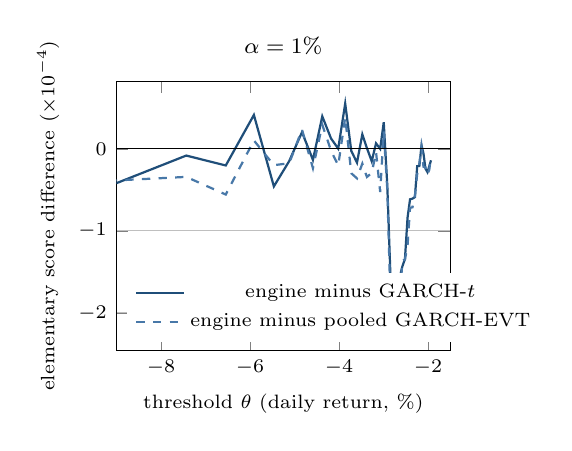
\begin{tikzpicture}
\begin{axis}[width=0.48\linewidth,height=5cm, xlabel={threshold $\theta$ (daily return, \%)}, ylabel={elementary score difference ($\times10^{-4}$)},
  title={$\alpha=1\%$}, xmin=-9, xmax=-1.5, ymajorgrids, legend style={font=\scriptsize,draw=none,at={(0.03,0.03)},anchor=south west},
  tick label style={font=\scriptsize}, label style={font=\scriptsize}, title style={font=\footnotesize}]
\addplot[npblue,thick] coordinates {(-15.879,-0.205) (-8.997,-0.418) (-7.431,-0.082) (-6.543,-0.203) (-5.911,0.413) (-5.462,-0.458) (-5.117,-0.149) (-4.830,0.203) (-4.584,-0.135) (-4.374,0.396) (-4.178,0.127) (-4.016,0.002) (-3.859,0.552) (-3.722,-0.026) (-3.594,-0.168) (-3.474,0.177) (-3.371,0.009) (-3.263,-0.151) (-3.166,0.067) (-3.073,0.000) (-2.993,0.324) (-2.913,-0.448) (-2.838,-1.619) (-2.765,-2.153) (-2.698,-1.874) (-2.632,-1.562) (-2.574,-1.432) (-2.516,-1.343) (-2.458,-0.839) (-2.402,-0.615) (-2.347,-0.607) (-2.292,-0.588) (-2.241,-0.211) (-2.192,-0.209) (-2.144,0.042) (-2.100,-0.057) (-2.055,-0.242) (-2.010,-0.284) (-1.969,-0.211) (-1.931,-0.140)};
\addplot[npmid,thick,dashed] coordinates {(-15.879,-0.193) (-8.997,-0.385) (-7.431,-0.342) (-6.543,-0.557) (-5.911,0.102) (-5.462,-0.199) (-5.117,-0.176) (-4.830,0.235) (-4.584,-0.236) (-4.374,0.293) (-4.178,-0.022) (-4.016,-0.203) (-3.859,0.383) (-3.722,-0.298) (-3.594,-0.360) (-3.474,-0.180) (-3.371,-0.343) (-3.263,-0.295) (-3.166,-0.039) (-3.073,-0.526) (-2.993,0.212) (-2.913,-0.496) (-2.838,-1.926) (-2.765,-2.079) (-2.698,-2.182) (-2.632,-1.837) (-2.574,-1.366) (-2.516,-1.347) (-2.458,-1.183) (-2.402,-0.718) (-2.347,-0.713) (-2.292,-0.569) (-2.241,-0.306) (-2.192,-0.174) (-2.144,0.023) (-2.100,-0.218) (-2.055,-0.227) (-2.010,-0.314) (-1.969,-0.254) (-1.931,-0.090)};
\addplot[black,thin] coordinates {(-9,0)(-1.5,0)};
\legend{engine minus GARCH-$t$, engine minus pooled GARCH-EVT}
\end{axis}
\end{tikzpicture}
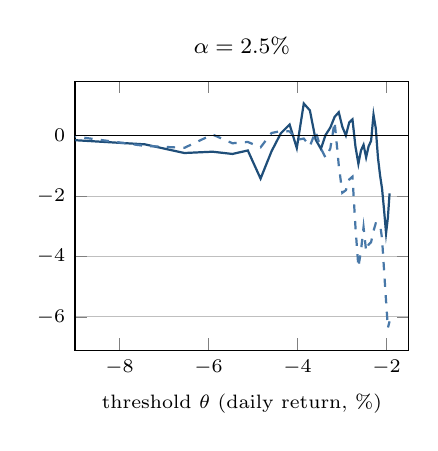
\begin{tikzpicture}
\begin{axis}[width=0.48\linewidth,height=5cm, xlabel={threshold $\theta$ (daily return, \%)},
  title={$\alpha=2.5\%$}, xmin=-9, xmax=-1.5, ymajorgrids,
  tick label style={font=\scriptsize}, label style={font=\scriptsize}, title style={font=\footnotesize}]
\addplot[npblue,thick] coordinates {(-15.879,-0.080) (-8.997,-0.151) (-7.431,-0.288) (-6.543,-0.575) (-5.911,-0.532) (-5.462,-0.606) (-5.117,-0.491) (-4.830,-1.423) (-4.584,-0.519) (-4.374,0.079) (-4.178,0.369) (-4.016,-0.412) (-3.859,1.062) (-3.722,0.836) (-3.594,-0.126) (-3.474,-0.440) (-3.371,0.017) (-3.263,0.266) (-3.166,0.620) (-3.073,0.775) (-2.993,0.293) (-2.913,0.007) (-2.838,0.435) (-2.765,0.539) (-2.698,-0.360) (-2.632,-0.930) (-2.574,-0.494) (-2.516,-0.305) (-2.458,-0.719) (-2.402,-0.350) (-2.347,-0.176) (-2.292,0.692) (-2.241,0.243) (-2.192,-0.729) (-2.144,-1.323) (-2.100,-1.754) (-2.055,-2.459) (-2.010,-3.227) (-1.969,-2.711) (-1.931,-1.910)};
\addplot[npmid,thick,dashed] coordinates {(-15.879,-0.036) (-8.997,-0.029) (-7.431,-0.340) (-6.543,-0.404) (-5.911,0.037) (-5.462,-0.252) (-5.117,-0.209) (-4.830,-0.388) (-4.584,0.087) (-4.374,0.152) (-4.178,0.141) (-4.016,-0.138) (-3.859,-0.097) (-3.722,-0.349) (-3.594,0.141) (-3.474,-0.426) (-3.371,-0.731) (-3.263,-0.426) (-3.166,0.464) (-3.073,-0.978) (-2.993,-1.892) (-2.913,-1.805) (-2.838,-1.451) (-2.765,-1.356) (-2.698,-3.018) (-2.632,-4.352) (-2.574,-3.815) (-2.516,-3.030) (-2.458,-3.818) (-2.402,-3.603) (-2.347,-3.527) (-2.292,-3.151) (-2.241,-2.900) (-2.192,-2.913) (-2.144,-2.935) (-2.100,-3.409) (-2.055,-4.461) (-2.010,-5.476) (-1.969,-6.361) (-1.931,-6.146)};
\addplot[black,thin] coordinates {(-9,0)(-1.5,0)};
\end{axis}
\end{tikzpicture}
\caption{Murphy diagrams for the VaR forecasts on the frontier rows: mean elementary quantile score of the accuracy layer minus that of GARCH-$t$ (solid) and of the pooled GARCH-EVT (dashed), against the threshold $\theta$. Negative values favor the accuracy layer. It is better on 70\% (GARCH-$t$) and 85\% (GARCH-EVT) of the grid at $\alpha=1\%$ and on 65\% and 85\% at $\alpha=2.5\%$; the competitors win in a band of thresholds near the typical VaR level, so the ranking is not uniform over all consistent quantile scores.}
\label{fig:murphy}
\end{figure}

\subsection*{All benchmarks on the canonical rows}
The GARCH-EVT comparison above is one row of a larger exercise (\texttt{job\_bench\_all.py}, result file \texttt{bench\_all\_results.json}): every model in the paper's comparison set is scored on the identical 221,600 test rows of the 200-name panel, through every statistic. GARCH-$t$, GJR-GARCH-skew-$t$, the two GARCH-EVT forms, the GAS and Taylor models and SAV-CAViaR are estimated per name on the estimation window; the FHS variants take the empirical quantiles of the GARCH-$t$ residuals (pooled across names, per name on the training window, or over a rolling 500-day window); EWMA is the RiskMetrics recursion with Gaussian quantiles; historical simulation is the rolling 500-day empirical return quantile. GAS and Taylor exist only at the two regulatory levels and enter the joint-score, dynamic-quantile and Murphy statistics. Table~\ref{tab:bench-pinball} gives the eleven-level pinball frontier, Table~\ref{tab:bench-fz0} the joint score, and Table~\ref{tab:bench-tests} the conditional-predictive-ability, dynamic-quantile, Murphy and win-rate statistics.

\begin{table}[htbp]
\centering
\begin{threeparttable}
\caption{Every benchmark on the frontier rows: eleven-level pinball edge over GARCH-$t$ by score region, engine head-to-head, and Model Confidence Set membership.}
\label{tab:bench-pinball}
\footnotesize
\begin{tabular}{lccccc}
\toprule
Model & Top $\mathrm{mk}_{63}$ decile & Deciles 1--9 & Overall & Engine vs model (top) & MCS \\
\midrule
Engine (accuracy layer) & $+2.48$ (10.08) & $-0.01$ (-0.25) & $+0.27$ (4.62) & --- &  \\
GARCH $+$ pooled body (no EVT) & $+2.98$ (10.48) & $+0.02$ (0.43) & $+0.35$ (5.35) & $-0.51$ (-9.04) & $\checkmark$ \\
GARCH(1,1)-$t$ & (reference) & (reference) & (reference) & $+2.48$ (10.08) &  \\
GJR-GARCH-skew-$t$ & $+0.16$ (0.60) & $-0.01$ (-0.13) & $+0.01$ (0.35) & $+2.32$ (9.70) &  \\
GARCH-FHS (pooled) & $-0.14$ (-2.45) & $-0.12$ (-4.39) & $-0.13$ (-4.62) & $+2.62$ (8.86) &  \\
GARCH-FHS (per name) & $+0.34$ (3.87) & $-0.27$ (-6.86) & $-0.20$ (-5.33) & $+2.15$ (9.67) &  \\
GARCH-FHS (rolling 500d) & $-0.75$ (-6.68) & $-0.03$ (-0.55) & $-0.11$ (-2.19) & $+3.21$ (10.22) &  \\
GARCH-EVT (pooled tail) & $-0.16$ (-2.69) & $-0.12$ (-4.55) & $-0.12$ (-4.89) & $+2.64$ (8.91) &  \\
GARCH-EVT (per name) & $+0.31$ (3.62) & $-0.22$ (-6.61) & $-0.16$ (-5.00) & $+2.18$ (9.63) &  \\
SAV-CAViaR & $+2.81$ (8.16) & $+0.08$ (1.60) & $+0.39$ (6.29) & $-0.33$ (-1.82) & $\checkmark$ \\
EWMA (RiskMetrics) & $-7.31$ (-9.91) & $-0.43$ (-3.54) & $-1.20$ (-8.39) & $+9.13$ (12.07) &  \\
Historical simulation (500d) & $+0.97$ (1.88) & $-1.98$ (-8.39) & $-1.65$ (-7.04) & $+1.53$ (4.46) &  \\
\bottomrule
\end{tabular}
\begin{tablenotes}\footnotesize
\item 200 names, 221,600 test rows, the rows of Table~2 of the paper. Edge $=$ (GARCH-$t$ pinball $-$ model pinball)/GARCH-$t$ pinball over the eleven-level grid, per-date Newey--West(10) DM in parentheses. The last column is the 90\% Model Confidence Set on the per-date eleven-level pinball series (T$_{\max}$, stationary bootstrap over dates, mean block 10, $B=1{,}000$).
\end{tablenotes}
\end{threeparttable}
\end{table}

\begin{table}[htbp]
\centering
\begin{threeparttable}
\caption{Every benchmark on the full-panel FZ0 rows.}
\label{tab:bench-fz0}
\footnotesize
\begin{tabular}{lcccccccc}
\toprule
& \multicolumn{4}{c}{$\alpha=1\%$} & \multicolumn{4}{c}{$\alpha=2.5\%$} \\
\cmidrule(lr){2-5}\cmidrule(lr){6-9}
Model & FZ0 & Breach & DM & MCS & FZ0 & Breach & DM & MCS \\
\midrule
Engine (accuracy layer) & 2.1465 & 1.04\% & --- & $\checkmark$ & 1.8486 & 2.78\% & --- & $\checkmark$ \\
Engine $+$ static shift (97.5\%) & 2.1465 & 1.04\% & 0.00 & $\checkmark$ & 1.8664 & 1.66\% & 2.57 &  \\
GARCH $+$ pooled body (no EVT) & 2.1411 & 1.32\% & -1.09 & $\checkmark$ & 1.8432 & 3.25\% & -1.54 & $\checkmark$ \\
GARCH(1,1)-$t$ & 2.1557 & 1.03\% & 4.94 &  & 1.8542 & 2.71\% & 5.50 &  \\
GJR-GARCH-skew-$t$ & 2.1505 & 1.02\% & 1.24 & $\checkmark$ & 1.8486 & 2.64\% & -0.02 & $\checkmark$ \\
GARCH-FHS (pooled) & 2.1557 & 1.14\% & 3.93 &  & 1.8598 & 3.00\% & 5.89 &  \\
GARCH-FHS (per name) & 2.1724 & 1.24\% & 4.91 &  & 1.8624 & 3.08\% & 5.35 &  \\
GARCH-FHS (rolling 500d) & 2.1847 & 1.10\% & 6.61 &  & 1.8611 & 2.50\% & 4.10 &  \\
GARCH-EVT (pooled tail) & 2.1551 & 1.06\% & 4.51 &  & 1.8583 & 2.89\% & 6.33 &  \\
GARCH-EVT (per name) & 2.1693 & 1.13\% & 5.14 &  & 1.8596 & 2.93\% & 5.36 &  \\
GAS-FZ (PZC) & 2.2324 & 0.92\% & 9.91 &  & 1.8990 & 2.53\% & 8.78 &  \\
ES-CAViaR (Taylor) & 2.1647 & 0.98\% & 3.76 &  & 1.8490 & 2.62\% & 0.13 & $\checkmark$ \\
EWMA (RiskMetrics) & 2.3211 & 1.61\% & 6.89 &  & 1.9035 & 2.73\% & 6.25 &  \\
Historical simulation (500d) & 2.2512 & 0.87\% & 6.34 &  & 1.9182 & 2.06\% & 5.28 &  \\
\bottomrule
\end{tabular}
\begin{tablenotes}\footnotesize
\item FZ0 is the zero-homogeneous Fissler--Ziegel joint (VaR, ES) loss, lower is better; DM $>0$ means the row model scores worse than the accuracy layer (per-date Newey--West(10)). ES: closed forms for the $t$ and Gaussian entrants; an exact substitution integral for the skew-$t$; empirical tail means for HS and FHS; McNeil--Frey closed form for GARCH-EVT; the FZ0-estimated dynamic pair for GAS and Taylor (the GAS fit of record is this run's); the converged integral of the monotonized curve for the engine (Section~2.2 of the paper), and a 20-node integral for the body, which has no quantile below its lowest fitted level. The static-shift row is the split-conformal shift of earlier versions, estimated on the body's calibration errors; Stage~4 now uses the adaptive overlay of Section~5.1 of the paper. At 2.5\% the engine, the body, GJR-GARCH-skew-$t$ and the Taylor model form a tie group (FZ0 1.8432--1.8490, $|$DM$|\le1.54$), reported as a group rather than an order. SAV-CAViaR produces no ES and is absent here. MCS: 90\% Model Confidence Set on the per-date FZ0 series.
\end{tablenotes}
\end{threeparttable}
\end{table}

\begin{table}[htbp]
\centering
\begin{threeparttable}
\caption{Conditional predictive ability, dynamic quantile test, Murphy diagrams and win rates for every benchmark against the accuracy layer.}
\label{tab:bench-tests}
\footnotesize
\begin{tabular}{lcccccccc}
\toprule
& \multicolumn{2}{c}{CPA vs engine} & \multicolumn{2}{c}{DQ pass rate} & \multicolumn{2}{c}{Murphy: engine better} & \multicolumn{2}{c}{Engine win rate} \\
\cmidrule(lr){2-3}\cmidrule(lr){4-5}\cmidrule(lr){6-7}\cmidrule(lr){8-9}
Model & Wald $\chi^2_2$ & slope $t$ & 1\% & 2.5\% & 1\% & 2.5\% & top decile & overall \\
\midrule
Engine $+$ static shift (97.5\%) & --- & --- & 86\% & 84\% & 0\% & 45\% & --- & --- \\
GARCH $+$ pooled body (no EVT) & 97.2 & -10.1 & 69\% & 54\% & 82\% & 72\% & 12\% & 26\% \\
GARCH(1,1)-$t$ & 73.6 & 8.6 & 84\% & 68\% & 70\% & 65\% & 74\% & 62\% \\
GJR-GARCH-skew-$t$ & 87.7 & 9.5 & 90\% & 77\% & 48\% & 40\% & 72\% & 62\% \\
GARCH-FHS (pooled) & 63.4 & 7.2 & 78\% & 60\% & 88\% & 85\% & 73\% & 62\% \\
GARCH-FHS (per name) & 80.3 & 4.6 & 73\% & 55\% & 92\% & 90\% & 72\% & 62\% \\
GARCH-FHS (rolling 500d) & 138.2 & 12.0 & 84\% & 82\% & 85\% & 50\% & 74\% & 64\% \\
GARCH-EVT (pooled tail) & 64.5 & 7.5 & 83\% & 62\% & 85\% & 85\% & 74\% & 62\% \\
GARCH-EVT (per name) & 68.2 & 5.2 & 82\% & 60\% & 78\% & 72\% & 72\% & 62\% \\
SAV-CAViaR & 2.6 & -0.2 & 78\% & 66\% & 80\% & 60\% & 52\% & 56\% \\
GAS-FZ (PZC) & --- & --- & 92\% & 82\% & 50\% & 78\% & --- & --- \\
ES-CAViaR (Taylor) & --- & --- & 78\% & 72\% & 70\% & 42\% & --- & --- \\
EWMA (RiskMetrics) & 172.6 & 13.8 & 29\% & 56\% & 95\% & 78\% & 83\% & 71\% \\
Historical simulation (500d) & 89.3 & -0.4 & 48\% & 51\% & 48\% & 60\% & 58\% & 72\% \\
\midrule
Engine (accuracy layer) & --- & --- & 86\% & 70\% & --- & --- & --- & --- \\
\bottomrule
\end{tabular}
\begin{tablenotes}\footnotesize
\item CPA: Giacomini--White Wald test of equal conditional accuracy of the model and the engine with instruments (1, lagged composite score percentile), Newey--West(10) over per-date sums, and the date-clustered $t$ of the slope of the loss differential (model minus engine) on the score; a positive slope means the engine's advantage grows with the score. DQ: Engle--Manganelli dynamic quantile test with four hit lags and the VaR, share of names passing at 5\%. Murphy: share of a forty-point return-space threshold grid on which the engine has the lower elementary quantile score. Win rate: share of test dates on which the date-averaged engine pinball is below the model's. Models with an entry only at the regulatory levels (GAS, Taylor) have no pinball-based columns.
\end{tablenotes}
\end{threeparttable}
\end{table}


\begin{table}[htbp]
\centering
\begin{threeparttable}
\caption{The ten-day extension against iterated benchmarks (main text, ten-day subsection). Direct multi-day model's pinball edge over each benchmark, $h=10$, both eras, on the purged rows of the ten-day sections.}
\label{tab:tenday}
\scriptsize\setlength{\tabcolsep}{3pt}
\begin{tabular}{lcccc}
\toprule
& \multicolumn{2}{c}{Design era, 2020--2024 test window} & \multicolumn{2}{c}{Holdout, mid-2008 to 2013} \\
\cmidrule(lr){2-3}\cmidrule(lr){4-5}
Benchmark & Edge \% (DM; NO) & Cov.\ 1\% / 2.5\% & Edge \% (DM; NO) & Cov.\ 1\% / 2.5\% \\
\midrule
$\sqrt{h}$-scaled GARCH-$t$ (paper) & $+1.41$ (6.8; 4.3) & 1.24 / 3.30 & $+0.52$ (0.09; -0.02) & 1.26 / 2.80 \\
Iterated-variance GARCH-$t$ & $+0.79$ (4.0; 2.7) & 1.03 / 2.85 & $+0.54$ (0.14; 0.15) & 1.23 / 2.74 \\
Simulated GARCH-$t$ paths & $+0.70$ (3.5; 2.5) & 1.20 / 2.93 & $+0.76$ (0.25; 0.20) & 1.44 / 2.79 \\
Bootstrapped filtered paths & $+0.51$ (2.5; 1.1) & 1.01 / 2.58 & $+0.81$ (0.25; 0.31) & 1.29 / 2.62 \\
Envelope, $\min$(direct, $\sqrt{h}$) & $+1.14$ (3.9; 2.4) & 0.94 / 2.45 & $+0.15$ ($-0.32$; 0.04) & 1.01 / 2.38 \\
Variance-ratio rescaling & $-0.12$ ($-1.7$; $-0.3$) & 0.97 / 2.44 & $+0.07$ (2.3; 2.0) & 1.23 / 2.79 \\
Direct model & --- & 1.13 / 2.80 & --- & 1.24 / 2.82 \\
\bottomrule
\end{tabular}
\begin{tablenotes}\footnotesize
\item Design era: 150 names, 164,850 test rows, 1,099 dates; holdout: 200 names, 278,808 rows, 1,486 dates. Edge $=$ (benchmark pinball $-$ direct pinball)/benchmark pinball over the eleven levels of the paper. Labels overlap (each row's target is the next ten days), so the DM statistic is computed on per-date mean loss differences with a Newey--West lag of 10; NO repeats it on every tenth test date (110 and 149 dates). Coverage is the share of rows whose realized ten-day return falls below the forecast quantile. Iterated-variance GARCH-$t$ uses the closed-form sum of the fitted GARCH variance forecasts over the ten days with the one-day $t$ shape; the path benchmarks simulate 4,000 ten-day paths per row from the fitted GARCH-$t$ with $t$ innovations or with residuals bootstrapped from the training window. The ratio of the iterated ten-day variance to $h$ times the one-day variance averages 1.07 in 2020, 1.11 in 2021, 1.06 in 2022, 1.12 in 2023, 1.11 in 2024 in the design era and 0.99 in 2008, 1.00 in 2009, 1.02 in 2010, 1.02 in 2011, 1.04 in 2012, 1.04 in 2013, which is why the $\sqrt{h}$ rule under-scales in the later era only. Holdout standard errors are roughly 3--6\% of loss, so the out-of-era accuracy comparison is uninformative; see \texttt{tenday\_diag\_results.json}. The envelope (the level-wise minimum of the direct and $\sqrt{h}$ curves, rearranged) and the variance-ratio rescaling (the direct curve rescaled by the square root of the iterated-to-$\sqrt{h}$ variance ratio) come from a rerun on the same rows, \texttt{tenday\_envelope\_results.json}, in which the $\sqrt{h}$ row reads $+1.39$ (DM 6.7) in era and $+0.51$ (DM 0.05) out of era. In 2008--2009 the envelope breaches at 1.61\% and 3.52\%, against 1.93\% and 3.99\% for $\sqrt{h}$ scaling and 2.15\% and 4.33\% for the direct model. Both constructions were run with predictions written beforehand; the envelope did not meet its two, and the rescaling is exploratory.
\end{tablenotes}
\end{threeparttable}
\end{table}


\begin{table}[htbp]
\centering
\begin{threeparttable}
\caption{Learner feature ablation (Section~4 of the paper). The Table~2 learner retrained with reduced state vectors; the score is computed as in the paper and is never a learner input.}
\label{tab:ablation}
\scriptsize\setlength{\tabcolsep}{3pt}
\begin{tabular}{lccccc}
\toprule
Learner & Top mk$_{63}$ & Top $|$sk$_{63}|$ & Top composite & Deciles 1--8 & Overall \\
\midrule
Full (logsig, $z_{t-1}$, $|z|_5$, sd$_{21}$, dn$_5$) & $+2.98$ (10.5) & $+2.78$ (9.8) & $+2.79$ (8.9) & $-0.20$ to $+0.11$ & $+0.35$ (5.3) \\
No dispersion (logsig, $z_{t-1}$, dn$_5$) & $+1.93$ (10.4) & $+1.78$ (9.9) & $+2.02$ (10.2) & $-0.40$ to $+0.08$ & $+0.14$ (2.3) \\
Scale only (logsig) & $+1.63$ (11.0) & $+1.56$ (10.6) & $+1.81$ (10.0) & $-0.43$ to $+0.12$ & $+0.12$ (2.4) \\
\bottomrule
\end{tabular}
\begin{tablenotes}\footnotesize
\item 200 CRSP names, 221,600 test asset-days, the rows of Table~2. Edge $=$ (GARCH-$t$ pinball $-$ learner pinball)/GARCH-$t$ pinball over the eleven levels, per-date DM with Newey--West lag 10 in parentheses. Against the full learner in the top mk$_{63}$ decile the no-dispersion learner loses $1.08\%$ (DM $-7.3$) and the scale-only learner $1.39\%$ (DM $-8.2$). Features: logsig is the log GARCH scale, $z_{t-1}$ the lagged standardized residual, $|z|_5$ its five-day mean absolute value, sd$_{21}$ its 21-day standard deviation, dn$_5$ the five-day share of down days. Result file \texttt{feature\_ablation\_results.json}; predictions in the script header.
\end{tablenotes}
\end{threeparttable}
\end{table}

\begin{table}[htbp]
\centering
\begin{threeparttable}
\caption{A state-adaptive parametric benchmark (Section~4 of the paper): GARCH-$t$ with a time-varying degrees-of-freedom law, on the rows of Table~2.}
\label{tab:arcd}
\scriptsize\setlength{\tabcolsep}{4pt}
\begin{tabular}{lcccc}
\toprule
Comparison & Top mk$_{63}$ decile & Top composite decile & Deciles 1--9 & Overall \\
\midrule
Adaptive-$\nu$ GARCH-$t$ over GARCH-$t$ & $+0.27$ (1.9) & $+0.03$ (0.8) & $+0.07$ (3.8) & $+0.10$ (3.8) \\
Learner over GARCH-$t$ (Table~2) & $+2.98$ (10.5) & $+2.79$ (8.9) & $+0.02$ (0.4) & $+0.35$ (5.3) \\
Learner over adaptive-$\nu$ GARCH-$t$ & $+2.72$ (9.7) & $+2.76$ (8.1) & $-0.05$ (-0.7) & $+0.26$ (3.4) \\
\bottomrule
\end{tabular}
\begin{tablenotes}\footnotesize
\item The benchmark keeps the paper's GARCH(1,1)-$t$ scale and replaces the constant $\nu$ by $\nu_t = 2.1 + \exp(h_t)$, $h_t = c + a|z_{t-1}| + b\,h_{t-1}$, an autoregressive conditional density in the spirit of \citet{hansen1994ARCD}, fitted by maximum likelihood on each name's training residuals with the scale held fixed; forecast quantile $\widehat\mu + \widehat\sigma_t\, t_\tau(\nu_t)/\sqrt{\nu_t/(\nu_t-2)}$. Median fitted $a = 0.11$, $b = 0.64$; median training log-likelihood gain over constant $\nu$ is 2.9 (48\% of names gain more than 3); the typical name's $\nu_t$ runs from 3.7 to 5.2 between its 10th and 90th percentiles. Edge $=$ (first model pinball $-$ second model pinball)/first, eleven levels, per-date DM with Newey--West lag 10. Result file \texttt{arcd\_bench\_results.json}; predictions in the script header.
\end{tablenotes}
\end{threeparttable}
\end{table}

\begin{table}[htbp]
\centering
\begin{threeparttable}
\caption{Synthetic truth (Section~4 of the paper): the estimator against the parametric model on its own scale, on panels simulated from a known model.}
\label{tab:synth}
\scriptsize\setlength{\tabcolsep}{4pt}
\begin{tabular}{llcccc}
\toprule
& & \multicolumn{2}{c}{Pinball DM} & \multicolumn{2}{c}{FZ0 difference ($\times10^{3}$)} \\
\cmidrule(lr){3-4}\cmidrule(lr){5-6}
Data generated by & Scale of both models & Overall & Top mk$_{63}$ decile & $1\%$ & $2.5\%$ \\
\midrule
GARCH-$t$ & GARCH-$t$ (true) & $-5.20$ & $-1.85$ & $+0.27$ & $+0.01$ \\
 & Beta-$t$-EGARCH & $10.17$ & $7.71$ & $-6.41$ & $-5.37$ \\
Beta-$t$-EGARCH & Beta-$t$-EGARCH (true) & $-4.29$ & $-1.41$ & $+0.29$ & $-0.18$ \\
 & GARCH-$t$ & $10.32$ & $8.14$ & $-1.62$ & $-1.61$ \\
\bottomrule
\end{tabular}
\begin{tablenotes}\footnotesize
\item Each panel is simulated per name from the named model, 200 names and 221,600 test rows. In each row the estimator (pooled shape learner and EVT tail on the stated scale) is compared with the parametric Student-$t$ model on the same scale. Pinball DM is the per-date Diebold--Mariano statistic of the estimator over that model on the eleven-level grid (positive favors the estimator); the FZ0 columns give mean FZ0 of the estimator minus that of the parametric model (negative favors the estimator), with the estimator's ES the converged integral and the parametric ES in closed form. Against the true model the estimator is slightly worse on pinball (by $0.02\%$ in both designs) and within $3\times10^{-4}$ on FZ0; against the misspecified scale's parametric tail it wins by $1.6$--$6.4\times10^{-3}$. The ES convention matters here: these gaps are smaller than the error of a 20-node midpoint ES, and under a correctly specified model the McNeil--Frey test with a 20-node ES rejects in $22.5\%$ of simulated samples at a nominal $5\%$ ($6\%$ with the exact ES). Result file \texttt{synthetic\_truth\_results.json}.
\end{tablenotes}
\end{threeparttable}
\end{table}

\subsection*{Expected-shortfall integral and an external transfer check}
Two items recorded for completeness. (i)~ES$_\alpha$ is the converged integral of the min-envelope curve (Section~2.2 of the paper). In one run on the same rows, replacing it by the GPD closed form of \citet{mcneilfrey2000} raises the accuracy layer's 2.5\% FZ0 from 1.8481 to 1.8508 (DM 4.2 in favour of the integral) and lowers its DM over GARCH-$t$ from 5.5 to 4.0; at 1\% the FZ0 rises from 2.1464 to 2.1487 (DM 2.5) and the DM over GARCH-$t$ falls from 4.7 to 4.3. The 20-node midpoint rule of earlier versions understated the engine's $|\ES|$ by $1.65\%$ at 1\% and $1.66\%$ at 2.5\% on average, for every one of the 200 names, and the rolling-window empirical rows of Table~4 of the paper by 4--5\%; those rows now use the exact tail mean. (ii)~As a transfer check outside finance, the same amortized pipeline scores a leakage-safe weighted scaled pinball of 0.269 (benchmark tier) on the M5 competition data.

\section{Frontier robustness: calendar overlap, family-wise error, and the universe rule}
This section collects the constructions summarized in Section~3 of the paper.

\paragraph{Calendar overlap and the pooled learner.} The design panels are split per name, $60/40$ in each name's own time index. In an unbalanced panel such a rule can place one name's training window on another name's test dates, so a pooled learner could meet a systemic event in training that a per-name model would meet only out of sample, the panel form of overlap leakage that purging and embargo address. Near-complete histories put the split points on almost the same date, so the channel is nearly degenerate here, and a strict calendar-time split closes it: each stage (each GARCH fit, the pooled learner, the GPD tail) is re-estimated strictly before 2020-01-01 and tested from that date for every name simultaneously. The frontier survives, with the top decile at $+2.47\%$ (per-date DM 6.22 over 1{,}258 dates; per-name split $+2.7\%$, DM 6.5) and the overall edge $+0.71\%$ (DM 1.87). The bottom decile is elevated at $+1.3\%$ because a 2020--22 test era leaves few calm cells, but the top decile roughly doubles each other cell. Inside the 2000--2013 holdout, re-estimating strictly before 2007-01-01 and testing on 2007--2013 removes the 2008 crisis from every training window; the pooled learner still wins overall ($+0.29\%$, per-date DM 3.08 over 1{,}762 dates) and the decile profile keeps its shape (top three deciles $+0.45$--$+1.04\%$ against $+0.06$--$+0.09\%$). The annual walk-forward refits the per-name GARCH on expanding data at each January-1 cutoff from 2020 to 2024, rebuilds the residuals and score, and retrains the learner; the top decile carries $+2.12\%$ at DM 4.41 while the overall edge is no longer detectable ($-0.22\%$, DM $-0.59$).

\paragraph{Family-wise error over the signal-decile grid.} The frontier grid spans three signals and ten deciles. Romano--Wolf step-down family-wise control over the full $3\times10$ grid takes studentized per-date mean edges per cell, a stationary bootstrap over dates that draws the same dates for every cell (mean block 10 days, $B=2{,}000$, block 20 as sensitivity), and one-sided step-down adjusted $p$-values. Nine of the thirty cells survive under both block lengths, all frontier cells: the top deciles of the three signals (mk$_{63}$ $t=9.4$, skew$_{63}$ $t=9.2$, jump$_5$ $t=5.1$, adjusted $p<0.001$), the ninth deciles of mk$_{63}$ (adjusted $p=0.022$) and skew$_{63}$, skew$_{63}$'s seventh, and jump$_5$'s U-shaped far cells. Mid-grid cells with an unadjusted $t$ near two lose significance under the adjustment.

\paragraph{The point-in-time universe.} The holdout's observation filter conditions on names present for most of the era, tilting the universe toward survivors. A point-in-time re-selection fixes the universe at the top 200 names by market capitalization as of Q1-2000, applies no minimum-history filter, and rides each delisting return to the end. On the 164 of 200 names that clear the symmetric fitting floors (36 dropped, 79 delisting returns ridden to the end), the overall edge is $+0.58\%$ at per-date DM 8.96 over 2{,}692 dates, the frozen design-era top bucket carries $+2.94\%$ at DM 6.6 ($5.9\%$ occupancy), and the bottom bucket is $+0.44\%$ (DM 5.4). The edge is larger than in the survivor-tilted holdout, so the observation filter biased the reported edge downward.

\section{Estimator schematic and evaluation panels}

\begin{figure}[h]
\centering
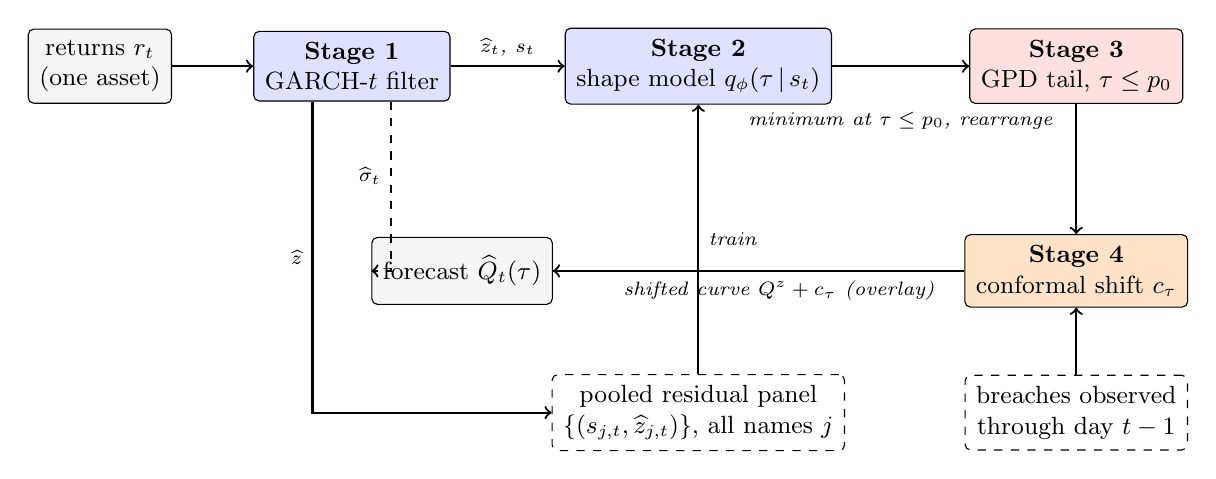
\begin{tikzpicture}[
  box/.style={draw, rounded corners=2pt, align=center, minimum height=8.5mm,
    inner sep=4pt, font=\small},
  lab/.style={font=\scriptsize\itshape, align=center},
  arr/.style={->, thick}]
\node[box, fill=gray!8]    (ret)   at (0,0)      {returns $r_t$\\(one asset)};
\node[box, fill=blue!12]   (garch) at (3.2,0)    {\textbf{Stage 1}\\GARCH-$t$ filter};
\node[box, fill=blue!12]   (shape) at (7.6,0)    {\textbf{Stage 2}\\shape model $q_\phi(\tau\,|\,s_t)$};
\node[box, fill=red!12]    (evt)   at (12.4,0)   {\textbf{Stage 3}\\GPD tail, $\tau\le p_0$};
\node[box, fill=orange!22] (conf)  at (12.4,-2.6){\textbf{Stage 4}\\conformal shift $c_\tau$};
\node[box, fill=gray!8]    (out)   at (4.6,-2.6) {forecast $\widehat{Q}_t(\tau)$};
\node[box, dashed, fill=white] (pool) at (7.6,-4.4) {pooled residual panel\\$\{(s_{j,t},\widehat z_{j,t})\}$, all names $j$};
\node[box, dashed, fill=white] (cal)  at (12.4,-4.4) {breaches observed\\through day $t-1$};
\draw[arr] (ret) -- (garch);
\draw[arr] (garch) -- node[lab, above] {$\widehat z_t$, $s_t$} (shape);
\draw[arr] (shape) -- node[lab, below=4.5mm] {minimum at $\tau\le p_0$, rearrange} (evt);
\draw[arr] (evt) -- (conf);
\draw[arr] (conf) -- node[lab, below, pos=0.45] {shifted curve $Q^{z}+c_\tau$ (overlay)} (out);
\draw[arr] ([xshift=-5mm]garch.south) |- node[lab, left, pos=0.25]
  {$\widehat z$} (pool.west);
\draw[arr] (pool.north) -- node[lab, right] {train} (shape.south);
\draw[arr] (cal.north) -- (conf.south);
\draw[arr, dashed] ([xshift=5mm]garch.south) |-
  node[lab, left, pos=0.22] {$\widehat\sigma_t$} (out.west);
\end{tikzpicture}
\caption{The residual-hybrid estimator as a pipeline (Section~2 of the paper). Solid arrows carry data; the dashed top arrow carries the conditional scale $\widehat\sigma_t$ that rescales the finished residual quantile curve. Dashed boxes are inputs shared across assets (the pooled panel that trains the amortized shape model) or observed as the forecasts are scored (the breaches behind the adaptive overlay).}
\label{fig:pipeline}
\end{figure}

\begin{table}[h]
\centering\small
\begin{threeparttable}
\caption{Sample flow across evaluation panels (Section~3 of the paper).}
\label{tab:sampleflow}
\footnotesize\setlength{\tabcolsep}{4pt}
\begin{tabular}{lllrrl}
\toprule
Panel & Source & Era & Names & Test obs & Role \\
\midrule
Design equity panel & CRSP/WRDS & 2014--2024 & 200 & 221{,}600 & frontier map, estimator development \\
Untouched-era holdout & CRSP/WRDS & 2000--2013 & 200 & 280{,}608 & frozen-spec replication \\
Subpanel & CRSP/WRDS & 2014--2024 & 140 & $\approx$155{,}000 & neural-network comparison, auxiliary checks \\
Cross-asset sweep & Bloomberg & through 2026 & 43 & \tnote{a} & frontier breadth \\
Country indices & Bloomberg & through 2026 & 26 & \tnote{a} & frontier breadth \\
\bottomrule
\end{tabular}
\begin{tablenotes}\footnotesize
\item[a] Frozen exhibits. Per-instrument windows vary and are documented instrument-by-instrument in the repository.
\end{tablenotes}
\end{threeparttable}
\end{table}

\section{What a top-decile score records}
The decomposition of Section~4 of the paper reads the top $\mathrm{mk}_{63}$ decile as a record of one recent large shock. Table~\ref{tab:anatomy} measures it on the 63-day window that defines each test row's score, with the canonical filter, panel and split (\texttt{tools/r63\_mk63\_anatomy.py}). Five predictions were written into the script before it ran. Three held: in the top decile one residual carries a median 97\% of the window's centered fourth-moment sum (predicted at least 60\%), removing it returns the median score to 1.07 (predicted below 3), and its timing is spread over the window (median 31 days, predicted 15 to 45). Two failed: the largest residual's median size in units of the window's own standard deviation is 6.1 (predicted at least 6.5), because the shock inflates the standard deviation it is measured against, and in deciles one to eight the largest term's median share is 0.39 (predicted below 0.30). The shock's size in conditional standard deviations of the filter and the dispersion of the other residuals were added after the first run, with no prediction attached. The holdout has smaller top-decile shocks and a smaller frontier (top-decile edge $+1.12\%$ against $+2.79\%$ on the composite score, Figure~1 of the paper).

\begin{table}[htbp]
\centering
\begin{threeparttable}
\caption{What the score records: the 63-day window behind each test row's $\mathrm{mk}_{63}$, by pooled decile of the score (medians).}
\label{tab:anatomy}
\footnotesize
% BEGIN anatomy body (generated by tools/make_r63_oa_tables.py)
\begin{tabular}{lcccccc}
\toprule
Decile & $\mathrm{mk}_{63}$ & Largest share & Share $>\tfrac12$ & Largest $|z|$ & SD of rest & $\mathrm{mk}_{63}$ without it \\
\midrule
\multicolumn{7}{l}{\emph{Panel A: 2014--2024 design panel (Table~2 rows, 221.6k asset-days)}} \\
1 & -0.27 & 0.21 & 0.00 & 2.3 & 0.91 & -0.47 \\
2 & 0.18 & 0.27 & 0.01 & 2.6 & 0.91 & -0.10 \\
3 & 0.56 & 0.31 & 0.03 & 2.8 & 0.92 & 0.16 \\
4 & 0.95 & 0.36 & 0.11 & 3.0 & 0.92 & 0.41 \\
5 & 1.43 & 0.41 & 0.26 & 3.2 & 0.92 & 0.66 \\
6 & 2.09 & 0.48 & 0.45 & 3.5 & 0.92 & 0.94 \\
7 & 3.12 & 0.59 & 0.68 & 4.0 & 0.93 & 1.18 \\
8 & 5.07 & 0.73 & 0.89 & 4.6 & 0.92 & 1.19 \\
9 & 9.24 & 0.87 & 0.98 & 5.7 & 0.89 & 1.19 \\
10 & 22.05 & 0.97 & 1.00 & 8.2 & 0.84 & 1.07 \\
\midrule
\multicolumn{7}{l}{\emph{Panel B: 2000--2013 holdout}} \\
1 & -0.42 & 0.19 & 0.00 & 2.2 & 0.89 & -0.59 \\
2 & -0.09 & 0.23 & 0.00 & 2.3 & 0.89 & -0.30 \\
3 & 0.18 & 0.27 & 0.00 & 2.5 & 0.89 & -0.09 \\
4 & 0.45 & 0.30 & 0.02 & 2.6 & 0.89 & 0.09 \\
5 & 0.75 & 0.34 & 0.07 & 2.8 & 0.88 & 0.28 \\
6 & 1.11 & 0.39 & 0.16 & 3.0 & 0.88 & 0.46 \\
7 & 1.60 & 0.45 & 0.36 & 3.2 & 0.88 & 0.65 \\
8 & 2.38 & 0.53 & 0.57 & 3.6 & 0.88 & 0.94 \\
9 & 4.05 & 0.69 & 0.85 & 4.1 & 0.86 & 0.98 \\
10 & 10.33 & 0.90 & 0.99 & 5.7 & 0.81 & 0.77 \\
\bottomrule
\end{tabular}
% END anatomy body
\begin{tablenotes}\footnotesize
\item Largest share: the share of the window's centered fourth-moment sum $\sum_i(\widehat z_i-\bar z)^4$ contributed by its single largest term. Share $>\tfrac12$: fraction of the decile's rows where that share exceeds one half. Largest $|z|$: that residual in conditional standard deviations of the GARCH-$t$ filter. SD of rest: standard deviation of the other 62 residuals, in the same units. $\mathrm{mk}_{63}$ without it: the score recomputed on the remaining 62 residuals with the same bias-corrected estimator.
\end{tablenotes}
\end{threeparttable}
\end{table}

\section{Top-decile edges against a robust reference}
Table~\ref{tab:attribution} scores every flexible model against two parametric references on the same rows, the paper's GARCH-$t$ and a Beta-$t$-EGARCH \citep{harvey2013dynamic} fitted per name by maximum likelihood with its own Student-$t$ tail (\texttt{code/paper/job\_bench\_all\_bteg.py}, frozen fits). The decile sort is the GARCH-$t$ score throughout. Against GARCH-$t$ both flexible models carry the frontier; against the robust reference both lose in the top decile, and only the models built on the robust scale keep a positive top-decile edge.

\begin{table}[htbp]
\centering
\begin{threeparttable}
\caption{Pinball edge (\%) against GARCH-$t$ and against Beta-$t$-EGARCH, per-date DM in parentheses. 200 CRSP names, 221,600 test rows.}
\label{tab:attribution}
\footnotesize\setlength{\tabcolsep}{4pt}
% BEGIN attribution body (generated by tools/make_r63_oa_tables.py)
\begin{tabular}{lcccc}
\toprule
& \multicolumn{3}{c}{Against GARCH-$t$} & Against Beta-$t$-EGARCH \\
\cmidrule(lr){2-4}\cmidrule(lr){5-5}
Model & Top decile & Deciles 1--9 & Overall & Top decile \\
\midrule
Pooled body (GARCH-$t$ scale) & $+2.94$ (10.56) & $+0.02$ (0.48) & $+0.35$ (5.33) & $-0.64$ (-2.59) \\
Accuracy layer (GARCH-$t$ scale) & $+2.44$ (10.18) & $-0.01$ (-0.20) & $+0.26$ (4.60) & $-1.16$ (-4.69) \\
SAV-CAViaR & $+2.81$ (8.16) & $+0.08$ (1.60) & $+0.39$ (6.29) & $-0.78$ (-3.70) \\
GJR-GARCH-skew-$t$ & $+0.16$ (0.60) & $-0.01$ (-0.13) & $+0.01$ (0.35) & $-3.52$ (-9.02) \\
GARCH-EVT (per name) & $+0.31$ (3.62) & $-0.22$ (-6.61) & $-0.16$ (-5.00) & $-3.37$ (-8.34) \\
GARCH-FHS (per name) & $+0.34$ (3.87) & $-0.27$ (-6.86) & $-0.20$ (-5.33) & $-3.34$ (-8.35) \\
Beta-$t$-EGARCH, Student-$t$ tail & $+3.56$ (8.80) & $+0.38$ (5.73) & $+0.74$ (9.37) & (reference) \\
Pooled body (Beta-$t$-EGARCH scale) & $+3.92$ (9.43) & $+0.35$ (7.06) & $+0.75$ (10.55) & $+0.37$ (2.66) \\
Accuracy layer (Beta-$t$-EGARCH scale) & $+3.82$ (9.27) & $+0.29$ (5.95) & $+0.69$ (9.69) & $+0.27$ (2.04) \\
\bottomrule
\end{tabular}
% END attribution body
\begin{tablenotes}\footnotesize
\item Edge $=$ (reference pinball $-$ model pinball)/reference pinball over the eleven-level grid; per-date Newey--West(10) DM. This run reproduces the GARCH-$t$ references of Table~OA.10 up to the seeding of the gradient-boosting early-stopping split (pooled body $+2.94\%$ here against $+2.98\%$ there).
\end{tablenotes}
\end{threeparttable}
\end{table}



\section{Detail moved from the main text}\label{sec:moved}

The paragraphs below were in the main text through R63 and moved here, unchanged except for cross-references, to shorten the paper. Each heading names the subject; the main text keeps a short pointer.

\subsection*{The ten-day horizon}
The multi-day results come from a direct amortized model trained on
$h$-day cumulative returns; the residual-hybrid of Algorithm~1 of the paper is a
one-day architecture, and no ten-day claim attaches to it. At the FRTB
ten-day liquidity horizon (CRSP 2014--2024) its pinball edge over
$\sqrt{h}$-scaled GARCH grows from $\sim$0.4\% at $h=1$ to $\sim$1.4\% at
$h=10$ and holds in the 2020--2022 stress window (Figure~OA.3). About half of that edge is the scaling rule itself. The
$\sqrt{h}$ rule holds the one-day variance flat across the window, while
the fitted GARCH variance mean-reverts toward an unconditional level that
sits $6$--$12\%$ above $h$ times the one-day variance in every year of
the 2020--2024 test window; against a GARCH-$t$ whose variance is
iterated through the window the direct model's edge is $0.8\%$ (DM 4.0),
against simulated GARCH-$t$ paths $0.7\%$ (DM 3.5), and against
bootstrapped filtered paths $0.5\%$ (DM 2.5, and 1.1 on non-overlapping dates), on the same rows. The
ten-day tail advantage is real in that era but does not survive the
pre-committed 2000--2013 rerun, where the fitted term structure is flat
(iterated ten-day variance within $2\%$ of $h$ times the one-day
variance in 2008--2009): out of era the two methods tie on accuracy
(direct edge $+0.52\%$, DM 0.09); against the iterated benchmarks the
point estimate is the same $0.5$--$0.8\%$ as in era, but with DM at most
0.3, because per-date loss differences through 2008 are far noisier; and the calibration
verdict reverses, with $\sqrt{h}$-scaled GARCH-$t$ almost exactly
calibrated through the crisis while the direct tail under-states it. A
level-wise minimum of the two curves does not repair this. In 2008--2009
it breaches at 1.61\% and 3.52\% against the 1\% and 2.5\% targets, closer
to nominal than $\sqrt{h}$ scaling (1.93\% and 3.99\%) but short of it, and
in era it costs 1.1\% of pinball against the direct model (DM 3.9), so we
do not recommend it. Rescaling the direct curve by the fitted variance term
structure ties the direct model in era (DM $-1.7$; $-0.3$ on
non-overlapping dates) with breach rates nearer nominal (0.97\% and
2.44\%) and loses to it out of era (DM 2.3); we record it as exploratory.
The ten-day evidence is therefore mixed; the benchmark
table is Table~OA.13.

\subsection*{Raw versus $\nu$-relative score}
The score's content could reflect model-relative
misspecification, departure from each name's own fitted $t_{\nu_i}$, or
the absolute level of recent tail activity. Converting each
mk$_{63}$ into a percentile of the simulated null of 63-window kurtosis
under the name's fitted $t_{\nu_i}$ leaves the frontier essentially
unchanged (top decile $+3.0\%$, DM 8.5, against $+2.98\%$, DM 10.5 raw).
The normalization is nearly rank-preserving, however (Spearman $0.97$, $82\%$
top-decile overlap), so it cannot by itself separate the two.

A discriminating test instead favors the raw-tail-activity reading.
In a within-date cross-sectional (Fama--MacBeth) regression of the
per-observation edge on the raw score and the $\nu$-relative percentile,
the raw score carries the predictive content ($t=7.8$), while the $\nu$-relative percentile has significantly negative incremental content ($t=-5.2$). Double-sorting agrees. The top-raw-kurtosis-quintile edge falls from $+1.9\%$ for the most fat-tailed (low-$\nu$) names to $+1.5\%$ for the thinnest-tailed, and observations high in the $\nu$-relative score but not in raw kurtosis carry no edge ($+0.3\%$, DM $0.5$). The signal is thus the absolute level of recent tail activity rather than
a per-name $\nu$-normalized surprise. The signal still measures shape
stress relative to the fitted model, since $\mathrm{mk}_{63}$ is computed on the
standardized residuals the model treats as stationary $t_\nu$.
Elevated values flag states in which the realized residual shape is
heavier or more asymmetric than the fitted law typically produces. A correctly specified low-$\nu$ $t_\nu$ can itself generate high realized kurtosis, which is why the score is treated as an indicator of stress and makes no claim to be a specification test (Section~2.5 of the paper). The data reject the finer per-name normalization. A plausible reason is that a name's fitted $\nu$ is estimated from the same residuals and a low value is itself a symptom of the tail activity that matters, so dividing it out removes part of the signal.

\subsection*{FZ0 on the large-cap sandbox subset}
On the
large-cap sandbox subset used to fix the score's orientation, a
Gaussian-innovation GARCH is significantly worst at both the 2.5\% and 1\%
levels (DM 5.4 and 6.0): under a jointly consistent score, Gaussian innovations
are clearly inadequate. Among the fat-tailed entrants the FZ0 differences on
large caps are small ($|$DM$|<1.4$), the frontier's own prediction that the
shape edge is flat on well-behaved names. On a high-kurtosis subset the ordering favors the shape-aware forecaster, directionally but not significantly at that width. The pre-specified full-panel run, reported next, settles the magnitudes on the residual-hybrid's own forecasts.

\subsection*{Why the joint-score edge is flat across deciles}
Dropping the EVT branch and scoring the pooled body alone, the body beats the accuracy layer in the top decile by 0.068 at 1\% (DM $-6.4$) and 0.060 at 2.5\% (DM $-6.8$), and ties it in the other nine deciles (0.002 and 0.001, DM 0.4 and 0.2). The pooled GPD is unconditional, so it sits at a fixed level in standardized-residual terms, $-2.55$ at 1\% and $-1.88$ at 2.5\%, while the body pulls its own tail quantile in from $-2.53$ to $-2.25$ across the deciles as the score rises, and the minimum of the two therefore overrides the body by a margin that widens from 0.19 to 0.52. Anchoring the same GPD to each row's own body quantile at the splice level, under a rule fixed before the run, removes the top-decile deficit (DM $+0.1$ against $-6.6$ for the unconditional tail at the same splice level) and raises the 97.5\% breach rate from 2.78\% to 3.09\%. The unconditional tail therefore buys about 0.3 points of 97.5\% coverage at a cost of 0.06 to 0.07 in top-decile FZ0 and 0.013 to 0.019 overall, and the paper keeps it for the coverage.

\subsection*{Direct ES calibration backtests}
Because exception counts test VaR and not ES,
two direct ES calibration backtests, the exceedance-residual test of \citet{mcneilfrey2000} and the $Z_2$ statistic of \citet{acerbi2014backtesting}, complement the jointly consistent FZ0 loss above. \citet{noldeziegel2017elicitability} and \citet{bayer2022esr} draw the
distinction between backtesting the calibration of an ES forecast and comparing
forecasts through a joint score. Both are computed on the residual-hybrid's own min-envelope forecasts over the same $200$-name panel, with a stationary block bootstrap over the $1{,}108$ test dates . The Gaussian filter is worst on each ES metric, and among the fat-tailed entrants no single model dominates each diagnostic. The residual-hybrid has the $Z_2$ closest to zero at $1\%$ and ties GARCH-$t$ at $2.5\%$, and the residual-hybrid and GARCH-$t$ are the two models that pass the $1\%$ Kupiec test. On the exceedance residual the residual-hybrid is closest to zero at $1\%$ and FHS, which targets the empirical tail directly, at $2.5\%$. Neither test rejects the residual-hybrid's ES at either level (exceedance residual $p=0.38$ and $0.58$, Table~OA.5), nor under the annual refits ($p=0.21$ and $0.33$), while GARCH-$t$'s $1\%$ ES is rejected as not severe enough ($p<0.001$). On the 2000--2013 holdout the verdict depends on the direction of the error. At $1\%$ the test rejects every construction, GARCH-$t$'s ES as not severe enough (mean exceedance residual $-0.17$) and the residual-hybrid's and FHS's as too severe ($+0.15$ and $+0.12$); at $2.5\%$ the residual-hybrid passes ($p=0.48$) and GARCH-$t$ is rejected ($p=0.02$). These verdicts require an accurate ES: with the 20-node midpoint ES of earlier versions, the exceedance-residual test rejects a correctly specified model in 22.5\% of simulated samples at a nominal 5\% (Table~OA.16). The comparative result is the FZ0 loss, where the edge over GARCH-$t$ and FHS is significant at both levels.

\subsection*{The implicit quantile network, estimator choice, and relation to GBC}
\emph{The neural implicit quantile network (IQN), the network at the core of GBC.} A
$\tau$-conditioned network
in the factorized form of \citet{dabney2018iqn} and
\citet{polson2023gbc},
\begin{equation}
H_\phi(s,\tau) \;=\; g\big(\psi(s)\circ c(\tau)\big),
\qquad
c_j(\tau) = \mathrm{ReLU}\Big(\textstyle\sum_{i=1}^{n_c}
\cos(\pi i \tau)\, w_{ij} + b_j\Big),
\label{eq:oaiqn}
\end{equation}
where $\circ$ is elementwise multiplication, $c(\tau)$ is a cosine embedding of the level with $n_c=64$ features, and $g,\psi$ are two-layer ReLU feed-forward nets of width 192 (128 in the untuned run) acting on the level embedding and on the standardized state respectively. The tuned variant uses tail-aware $\tau$-sampling, monotone rearrangement of the $\tau$-curve, and a conformal shift. The tail-aware sampling, $\lambda = \tfrac12\,U(0,1) + \tfrac12\,\mathrm{Beta}(0.3,0.3)$, was set once, before the tuned run, so that about a tenth of the training levels fall below 2.5\% against 2.5\% under uniform sampling; the mixture and the Beta parameters were not tuned on any test data. It answers the untuned run, whose 99\% breach rate was 3.2\% under uniform sampling, and the tuned IQN row of Table~5 of the paper is a design revision made after that run and evaluated on a later sub-window. The trade-off between the two estimators is set out under \emph{Estimator choice} below.

\emph{How training works.} The network minimizes the empirical version
of equation~(3) of the paper by stochastic gradient descent, each example
drawn at a fresh level $\tau_{jt}\sim\lambda$ each epoch, so one set of
weights carries the entire quantile curve. Training runs for a fixed budget of 12{,}000 minibatch steps (Adam, batch 512, rate $10^{-3}$; 6{,}000 in the untuned run) with no early stopping. Monotone rearrangement and the conformal shift
are applied \emph{after} training, and the whole pipeline is refit on
the annual walk-forward schedule using only past data. Layer sizes,
learning rates, and seeds are reported in the replication package.

\noindent\emph{Estimator choice.} The two estimators minimize the same loss over different index sets. The trees solve $\min \sum_{k}\sum_{i}\rho_{\tau_k}(\widehat{z}_i - q_k(s_i))$ on a fixed grid $\{\tau_k\}$, one model per level, while the network solves $\min_\phi \sum_i \mathbb{E}_{\tau\sim\lambda}\, \rho_\tau(\widehat{z}_i - H_\phi(s_i,\tau))$, one model for the continuum. At the fixed regulatory levels the trees are preferable: best point accuracy and no GPU, with the grid made monotone by rearrangement. The network learns one continuous conditional quantile map at a measured cost of $\sim$0.75\% in point accuracy. The two share each upstream and downstream stage of equation~(5) of the paper, so swapping one for the other changes a single component of the pipeline.

\noindent\emph{Relation to generative Bayesian computation.} Relative to the generative Bayesian computation of \citet{polson2023gbc}, the downside-risk target changes the estimator in five ways, each introduced above. The sampling measure $\lambda$ is tail-weighted rather than uniform, because uniform sampling starves the extreme levels that downside risk depends on. The object modeled is the GARCH-standardized residual rather than the raw return, so that the conditional-scale dynamics the parametric model already estimates well are kept. Beyond the training support, extrapolation is handed to the GPD tail equation~(4) of the paper rather than to the learner. The conformal stage adds a coverage correction driven by realized breaches. And the amortization runs across the real cross-section of hundreds of assets instead of across simulations of a single model, which is what produces the cold-start forecasts and transfer results. When such machinery improves on the parametric filter is not a question generative computation addresses, and the score of Section~2.5 of the paper is built to answer it.

\subsection*{The filter window and the calibration split}
One further
implementation gap: the first-stage
GARCH is fit on the full pre-test history, so the calibration errors
are held out from the shape learner and the EVT tail but not from the
filter. The accuracy-layer comparisons never read the calibration split
and share their filter with the benchmark, so their information sets
match. The adaptive overlay reads only breaches already observed in the test period, so no reported forecast reads the calibration split. Re-estimating with the filter stopped at the calibration boundary leaves the accuracy advantage intact (DM 5.0 and 5.1). The strict estimator's gap to the full-window benchmark ($-0.7$, $-2.6$) matches that benchmark's own margin over its short-window twin (2.8, 3.8), so the gap is the cost of a quarter less estimation data and shows no leakage.

\subsection*{The ES integral}
The body branch is the minimum on about 40\% of tail nodes. ES$_\alpha$ is the integral of equation~(5) of the paper over $(0,\alpha]$, computed to convergence: the body is interpolated across sixty fitted levels on $[\alpha/40,\alpha]$, the GPD branch is evaluated exactly at each of 2{,}000 nodes, and below $\alpha/40$, where the GPD quantile diverges, its integral is taken in closed form. A 20-node midpoint rule, used in earlier versions, understates the engine's $|\ES|$ by about 1.6\% for every one of the 200 names and distorts the ES backtests . With the GPD closed form of \citet{mcneilfrey2000} in place of the integral, the accuracy layer's FZ0 is significantly worse at both levels (DM 2.5 at $1\%$ and 4.2 at $2.5\%$) and its margin over GARCH-$t$ at $2.5\%$ narrows from DM 5.5 to 4.0 . The splice level is immaterial ($p_0\in\{1.5\%,2.5\%,5\%\}$: DM 4.5--4.7 at the $1\%$ level and 4.2--5.5 at $2.5\%$).

\subsection*{The composite score on the 2000--2013 holdout}
As
a post-hoc check, the composite score also replicates on this holdout.
Its top decile carries $+1.12\%$ (DM 2.51), marginally above its kurtosis
component ($+1.04\%$, DM 2.16, on the residual-hybrid learner; the frozen returns-space learner of Section~4 of the paper gives $+0.89\%$ at the same DM), and $+0.71\%$ (DM 2.08) under the
expanding prior-only cutoff. Because the composite was not the rule frozen at the time, this is replication on an already-examined sample, not a frozen-specification test.

\subsection*{Choice of scoring function}
\emph{Choice of scoring function.} We score by pinball, a consistent scoring function for the quantile \citep{gneiting2011}, at the decision-relevant levels rather than by a global proper scoring rule, for three reasons. (a)~The continuous ranked probability
score (CRPS), the proper scoring rule for the whole distribution \citep{gneitingraftery2007}, is exactly the integral of the pinball loss over all
levels, $\mathrm{CRPS}(F,y) = 2\int_0^1 \rho_\tau(y - F^{-1}(\tau))\,
d\tau$ \citep{gneitingranjan2011}. Scoring by CRPS therefore weights
quantile levels uniformly, so a 1\% tail occupies 1\% of the
integral. The quantile-weighted CRPS of \citet{gneitingranjan2011} reweights the levels for this reason, and scoring at fixed levels is its point-mass case. Downside
risk lives at fixed regulatory levels ($\tau \in \{0.01, 0.025\}$), and
the models in this paper differ almost entirely in the tail, and CRPS
would average those differences away against a body where all
competitors agree. For the same reason, training uses tail-weighted $\tau$-sampling. (b)~Expected Shortfall is not elicitable
on its own \citep{gneiting2011} (no loss function is minimized by the true ES alone), but
the pair $(\VaR,\ES)$ is, under the joint scoring functions of
\citet{fissler2016}, whose zero-homogeneous member, the FZ0 loss of \citet{patton2019}, is the one Section~5 of the paper uses. The FZ-scored re-evaluation of the comparison set is an extension specified in advance (Section~5 of the paper). (c)~Likelihood is
unavailable by design: several competitors have no tractable density, and likelihood scores
would silently exclude them. Each benchmark is estimated by its own conventional criterion: Student-$t$ or skew-$t$ likelihood for the GARCH family, empirical residual quantiles for HS and FHS, FZ0 for the two dynamic-ES models of Section~5 of the paper, and pinball for CAViaR and for the shape learners. All are then scored out of sample by the same pinball and FZ0 losses, so a model fitted on the evaluation loss carries an in-sample advantage that the out-of-sample comparison tests.

\subsection*{Distribution-free conditional quantiles, GBC, and conformal prediction}
The nonparametric family estimates $Q_\phi(\tau \mid s_t)$ directly by pinball-loss empirical risk minimization (ERM) \citep{koenker1978, steinwart2011}. Its two members here are gradient-boosted quantile trees (GBM) \citep{friedman2001} and the implicit quantile network of \citet{dabney2018iqn}, the architecture at the core of GBC \citep{polson2023gbc, nareklishvili2025gqbp}, itself in the generalized-Bayes tradition of \citet{jiang2008gibbs} and \citet{bissiri2016general}. In the IQN the quantile level $\tau$ is itself fed into the network, so one set of weights outputs the whole quantile curve rather than one grid point at a time.

Trained on observed state and residual pairs, GBC's quantile generator is a conditional quantile network, so the forward simulator of the original method is not needed and the same object applies to observational time series; Section~2.3 of the paper records how the downside-risk target changes it. The GBM is the shape model used throughout, and the IQN is retained as a benchmark. Distribution-free finite-sample coverage comes from split-conformal prediction \citep{vovk2005, lei2018, romano2019cqr}, which shifts a predicted quantile by an order statistic of held-out calibration errors so that marginal coverage holds under exchangeability with no distributional model. Adaptive conformal inference \citep{gibbs2021aci} replaces the fixed shift by an online update whose long-run coverage holds under arbitrary distribution shift, at the cost of the finite-sample guarantee. \citet{barber2023} bound the coverage loss when exchangeability fails, the case for time-ordered residuals.

\subsection*{The frontier across universes}
Table~\ref{tab:universes} is the cross-market table of Section~4.2 of the paper.

\begin{table}[htbp]
\centering
\begin{threeparttable}
\caption{The frontier across universes. Ratio $=$
nonparam/GARCH-$t$ pinball ($<1$: nonparametric wins). All fits
standalone per asset except where noted.}
\label{tab:universes}
\footnotesize\setlength{\tabcolsep}{4pt}
\begin{tabular}{llccl}
\toprule
Universe & Segment & Ratio & Resid.\ kurt. & Significance \\
\midrule
FX (24 pairs) & majors (7) & 1.019 & 39 & GARCH, pooled DM $-13.7$ \\
 & EM (10) & 1.013 & 8 & GARCH, pooled DM $-9.5$ \\
 & crisis (7) & 0.973 & $\sim$1915 & nonparam, pooled DM $4.12$ \\
 & \quad USDARS & 0.880 & 3298 & DM $2.86$, $p=.002$ \\
 & \quad USDEGP & 0.857 & 1920 & DM $3.80$, $p=.0001$ \\
\midrule
Country indices (26) & developed (8) & 1.007 & 4.7 & 0 nonparam wins \\
 & emerging (10) & 1.012 & 5.3 & 0 nonparam wins \\
 & frontier (8) & 0.993 & 10.0 & 4 significant wins\tnote{a} \\
\midrule
Cross-asset (43) & vol indices & $\sim$0.987 & 32.8 & 3/3 significant \\
 & Baltic freight & 0.846 & --- & DM $9.4$ (calib.\ fails) \\
 & IG credit OAS & 0.960 & --- & DM $2.3$ (indep.\ fails) \\
\multicolumn{5}{l}{\quad 13/43 significant wins overall, corr(log kurt, edge) $= 0.43$} \\
\midrule
Korea 2026 (23) & all types & 1.01--1.12 & 4--13 & GARCH wins all, DM $-2.5$ to $-5$ \\
\bottomrule
\end{tabular}
\begin{tablenotes}\footnotesize
\item[a] Sri Lanka (DM 3.20), Kenya (3.52), Pakistan (2.38), Nigeria (2.06). Exploratory: only Kenya survives the 93-comparison
familywise adjustment (Table~OA.4). Cross-index corr(log residual kurtosis, edge) $= 0.53$.
Philippines is the exception (GARCH wins despite kurtosis 13.6),
illustrating that kurtosis is neither necessary nor sufficient.
\end{tablenotes}
\end{threeparttable}
\end{table}

\section{The two-regime example}
\subsection*{A synthetic boundary check: when the frontier does
\emph{not} appear}\label{sec:toy}

Before the real data, a simulation with known truth (run once, seed
fixed) checks the formal results and, more usefully, delineates when
the frontier edge should \emph{fail} to appear. The data-generating
process is deliberately favorable to the score: unit-variance
Student-$t$ residuals whose degrees of freedom switch between a calm
regime ($\nu=12$) and a fat regime ($\nu=3$) under a persistent Markov
chain; forecasters see the trailing 63-day kurtosis score and compete
at $\tau \in \{0.01, 0.025\}$ (80{,}000 days; scale known, isolating
shape). First, the identity of Lemma~OA.1
verifies numerically: the regret integral and the Monte-Carlo regret
agree to five decimals ($3.5\times10^{-5}$ at $\tau=0.01$). Second, the
conformal shift moves realized coverage toward nominal on the held-out
split, as Proposition~1 of the paper promises. Third, and most instructive, the score-binned nonparametric
forecaster does
\emph{not} beat the fixed shape here: a single $t_{\widehat\nu}$
fitted on the mixture ($\widehat\nu = 6.8$) is nearly unbeatable at
these levels, with total regret under $0.5\%$ and no decile gradient.
Two mechanisms explain it. (i)~By
Lemma~OA.1 regret is \emph{quadratic} in the quantile
wedge, and at $\tau \ge 0.01$ the wedge between the fitted compromise
and either regime is small, so the regret from one fitted shape across
both regimes is second order. (ii)~The sample kurtosis of a $t_\nu$ law is a noisy statistic when
tails are fat: its usual moment-based asymptotic variance requires a
finite eighth moment ($\nu>8$), and the population kurtosis itself does
not exist for $\nu\le4$, so sixty-three observations cannot reliably
rank regimes that differ only in a static $\nu$. The jump and
asymmetry signals, whose top deciles independently survive familywise
control, corroborate the ordering, and a tail-index (Hill-type)
variant of the score is an obvious robustness extension. For the empirical sections this means the real-data top-decile edge of Section~4 of the paper
is not what averaging stationary fat tails produces in this
simulation (a fixed shape handles that configuration) and is consistent with \emph{local} shape breaks a single
fitted $\nu$ cannot straddle: asymmetry, jump clustering, and residual misfit
that co-move with the score. The Korea-2026 crash illustrates the same point from the opposite direction (a price crash without a residual outlier carries no edge), and it is why the score combines
kurtosis with asymmetry and a jump indicator rather than kurtosis
alone. (Simulation script \texttt{toy\_example.py} ships with the code
release.)


\section{Trading implications}
\textbf{Trading implications.} The universes where the nonparametric tail wins (crisis FX, volatility indices, credit spreads, frontier equities) are the desks where tail-shape-aware
sizing and hedging matter most. The \emph{direction} of the trade matters
as much as its location: a correct physical-measure tail forecast
does not by itself make bought crash insurance profitable, because the
crash risk premium can survive conditioning on a correct forecast.
A possible application is the opposite side, selling tail protection
with the model supplying tail control rather than alpha on the mean. The
paper evaluates no prices, premia, costs or trading outcomes, so the
application is untested here. The gating experiment provides no evidence that the score times
individual crash days, so its role there would be continuous tail-risk
measurement.




%% ===== CONCLUSION =====

\clearpage
\section{Proofs}\label{app:proofs}

The three formal results of Sections~2.2 and~2.4 of the paper are stated in the body; the complete arguments, with all regularity
hypotheses made explicit, are collected here. Throughout, $\rho_\tau(u)
= u(\tau - \mathbb{I}\{u<0\})$ and $q_F = F^{-1}(\tau) = \inf\{x:F(x)\ge
\tau\}$ is the lower generalized inverse.

\subsection*{Lemma OA.1 (pinball regret identity, standard) and proof}

\noindent\textbf{Lemma OA.1.} \emph{Let $Z \sim F$ with $\mathbb{E}|Z| < \infty$ and $q_F = F^{-1}(\tau)$, and let $S(q) = \mathbb{E}_F\,\rho_\tau(Z - q)$ be the expected pinball loss of forecasting the constant $q$, finite by the moment condition. Then for any $q$,}
\begin{equation}
S(q) - S(q_F) \;=\; \int_{q_F}^{q} \big(F(v) - \tau\big)\,dv \;\ge\; 0,
\label{eq:oaregret}
\end{equation}
\emph{with equality iff $F(u) = \tau$ for Lebesgue-almost each $u$ between $q_F$ and $q$.
If $F$ has density bounded as $0 < m \le f \le M$ on that closed interval,}
\begin{equation}
\tfrac{m}{2}\,(q - q_F)^2 \;\le\; S(q) - S(q_F) \;\le\;
\tfrac{M}{2}\,(q - q_F)^2 .
\label{eq:oaquadratic}
\end{equation}

\noindent\emph{Proof.} Assume $\mathbb{E}|Z|<\infty$, so
\[
S(q) = (1-\tau)\!\int_{(-\infty,q]}\!(q-z)\,dF(z)
\;+\; \tau\!\int_{(q,\infty)}\!(z-q)\,dF(z)
\]
is finite for every $q$, and $S$ is convex (an expectation of the
convex maps $q\mapsto\rho_\tau(z-q)$). For fixed $z$, $q\mapsto
\rho_\tau(z-q)$ is Lipschitz with constant $\max(\tau,1-\tau)$, so the
difference quotients $[\rho_\tau(Z-q')-\rho_\tau(Z-q)]/(q'-q)$ are
bounded by the integrable constant $\max(\tau,1-\tau)$; dominated
convergence justifies differentiating under the expectation wherever the
one-sided limits exist. Off the atoms of $F$,
\[
\frac{d}{dq}\,\rho_\tau(z-q) = \mathbb{I}\{z<q\}-\tau ,
\qquad\Longrightarrow\qquad
S'(q) = \mathbb{E}\,\mathbb{I}\{Z<q\}-\tau = F(q^-)-\tau,
\]
which equals $F(q)-\tau$ for all but countably many $q$. Since $S$ is
convex, hence absolutely continuous, the fundamental theorem of
calculus gives
\[
S(q)-S(q_F)=\int_{q_F}^{q}\big(F(u)-\tau\big)\,du,
\]
the countable atom set being Lebesgue-null; \emph{no continuity
hypothesis on $F$ is needed for this identity}. For nonnegativity,
note $q_F=\inf\{x:F(x)\ge\tau\}$ implies $F(u)\ge\tau$ for $u\ge q_F$
and $F(u)<\tau$ for $u<q_F$. If $q>q_F$ the integrand is $\ge0$ on
$[q_F,q]$, so the integral is $\ge0$; if $q<q_F$,
\[
S(q)-S(q_F)=\int_{q_F}^{q}\big(F(u)-\tau\big)\,du
=\int_{q}^{q_F}\big(\tau-F(u)\big)\,du\;\ge\;0 ,
\]
the integrand again $\ge0$ on $[q,q_F]$. Equality holds iff $F(u)=\tau$
for Lebesgue-a.e.\ $u$ between $q_F$ and $q$. Finally, if $F$ is
absolutely continuous with density $0<m\le f\le M$ on the interval
joining $q_F$ and $q$, then $F$ is continuous there, so $F(q_F)=\tau$
and $F(u)-\tau=\int_{q_F}^{u}f$; hence $m|u-q_F|\le|F(u)-\tau|\le
M|u-q_F|$, and integrating over the interval yields
$\tfrac{m}{2}(q-q_F)^2\le S(q)-S(q_F)\le\tfrac{M}{2}(q-q_F)^2$.
\hfill$\square$

\subsection*{Proof of Proposition~1 of the paper (split-conformal
validity)}

Let $k=\lceil(n{+}1)\tau\rceil$ and assume $1\le k\le n$ so that the
$k$-th order statistic $e_{(k)}=c_\tau$ of the $n$ calibration errors
$\{e_1,\dots,e_n\}$ exists; when $k=n+1$ (i.e.\ $\tau$ within $1/(n+1)$
of $1$) set $c_\tau=+\infty$, giving coverage $1$. Suppose the $n+1$
errors $e_1,\dots,e_{n+1}$ (calibration plus the test error
$e_{n+1}=z_{n+1}-\widehat q(\tau\mid s_{n+1})$) are exchangeable and
almost surely distinct. Then the rank $R$ of $e_{n+1}$ among the pooled
$n+1$ values is uniformly distributed on $\{1,\dots,n+1\}$. By
construction $\widetilde q(\tau\mid s_{n+1})=\widehat q(\tau\mid
s_{n+1})+c_\tau$, so
\[
\{z_{n+1}\le\widetilde q(\tau\mid s_{n+1})\}
=\{e_{n+1}\le c_\tau\}
=\{e_{n+1}\le e_{(k)}\}
=\{R\le k\},
\]
the middle equality using a.s.\ distinctness (with ties the middle
equality fails; e.g.\ if all $e_i$ are equal the event has probability
$1$, which can exceed the stated upper bound). Therefore
\[
\Pr\big(z_{n+1}\le\widetilde q(\tau\mid s_{n+1})\big)
=\Pr(R\le k)=\frac{k}{n+1}
=\frac{\lceil(n{+}1)\tau\rceil}{n+1}.
\]
Since $(n{+}1)\tau\le\lceil(n{+}1)\tau\rceil<(n{+}1)\tau+1$, dividing by
$n+1$ gives $\tau\le k/(n+1)<\tau+\tfrac1{n+1}$. The probability is over
the joint law of calibration and test points; the guarantee is
marginal, not conditional on $s_{n+1}$, because a single scalar shift
$c_\tau$ pooled across states cannot deliver state-conditional
coverage. \hfill$\square$

\subsection*{Proposition OA.1 (tail wedge, elementary) and proof}

\noindent\textbf{Proposition OA.1.} \emph{Let $Q_\nu(\tau)$ denote the $\tau$-quantile of the unit-variance
Student-$t$ with $\nu > 2$ degrees of freedom. For each pair
$\nu_2 > \nu_1 > 2$ there exists $\tau^*(\nu_1,\nu_2) \in (0, 1/2]$
such that $Q_{\nu_1}(\tau) < Q_{\nu_2}(\tau)$ for all $\tau < \tau^*$, and the wedge $|Q_{\nu_1}(\tau) - Q_{\nu_2}(\tau)| \to \infty$ as $\tau \downarrow 0$. Consequently, by Lemma~OA.1, a
forecaster committed to shape $t_{\nu_2}$ while the local truth is
$t_{\nu_1}$ pays regret bounded below by
$\tfrac{m}{2}\,(Q_{\nu_1}(\tau) - Q_{\nu_2}(\tau))^2$ at each level
$\tau < \tau^*$, where $m$ is the minimum of the true density on the
wedge interval.}

\noindent The bound is a fixed-level statement rather than a tail-limit one: because $m=m(\tau)$ shrinks as $\tau\downarrow0$, the certified regret stays positive at each level but does not grow into the tail, and in fact vanishes there.

\noindent\emph{Proof.} Fix $\nu>2$, so the $t_\nu$ law has finite variance and its
unit-variance version $Z=T_\nu\sqrt{(\nu-2)/\nu}$ is well defined. The
$t_\nu$ density is $\sim C_\nu|x|^{-(\nu+1)}$ as $|x|\to\infty$, so the
lower tail is regularly varying with index $-\nu$: $\Pr(T_\nu<-x)=
\tilde c_\nu x^{-\nu}(1+o(1))$. Unit-variance scaling multiplies the
constant, $\Pr(Z<-x)=c_\nu x^{-\nu}(1+o(1))$ with
$c_\nu=\tilde c_\nu((\nu-2)/\nu)^{\nu/2}$, and leaves the index $\nu$
unchanged. Writing $U(\tau)=|Q_\nu(\tau)|$ and inverting the regularly
varying tail \citep{embrechts1997} gives $\tau=c_\nu U(\tau)^{-\nu}
(1+o(1))$, hence $U(\tau)=(c_\nu/\tau)^{1/\nu}(1+o(1))$ as
$\tau\downarrow0$, i.e.\ $Q_\nu(\tau)=-(c_\nu/\tau)^{1/\nu}(1+o(1))$.
For $\nu_1<\nu_2$,
\[
\frac{|Q_{\nu_1}(\tau)|}{|Q_{\nu_2}(\tau)|}
=\frac{(c_{\nu_1}/\tau)^{1/\nu_1}}{(c_{\nu_2}/\tau)^{1/\nu_2}}\,(1+o(1))
=\text{const}\cdot\tau^{-(1/\nu_1-1/\nu_2)}(1+o(1))\;\longrightarrow\;\infty
\]
because $1/\nu_1>1/\nu_2$. Thus for all sufficiently small $\tau$ both
quantiles are negative with $|Q_{\nu_1}(\tau)|>|Q_{\nu_2}(\tau)|$, i.e.\
$Q_{\nu_1}(\tau)<Q_{\nu_2}(\tau)$, and the wedge
$|Q_{\nu_1}(\tau)-Q_{\nu_2}(\tau)|\to\infty$. The ordering therefore
holds for every $\tau<\delta$ for some $\delta>0$; putting
$\tau^*=\min(\delta,\tfrac12)$ gives $\tau^*\in(0,\tfrac12]$ as
asserted. (This establishes \emph{existence} of $\tau^*$; the actual
crossover $\tau_c$ where the ordering flips is not claimed here and is
located numerically in the crossover remark of the paper.) Under local truth
$t_{\nu_1}$, applying \eqref{eq:oaquadratic} with $q=Q_{\nu_2}(\tau)$ and
$q_F=Q_{\nu_1}(\tau)$ bounds the regret below by
$\tfrac{m}{2}(Q_{\nu_1}(\tau)-Q_{\nu_2}(\tau))^2$, with $m$ the minimum
of the $t_{\nu_1}$ density on the wedge interval. \hfill$\square$

\subsection*{Remark on the score ordering}
We state the score-ordering as an empirical regularity rather than a
theorem, and record here why no clean monotonicity theorem holds at the
deployable levels. The tail-wedge result (Proposition~OA.1)
orders a given pair of Student-$t$ tail indices only below a pair-specific
crossover level $\tau^*(\nu_1,\nu_2)$; it does not deliver monotonicity of
the wedge in the tail index at a fixed operational $\tau$. More
fundamentally, the innovations are unit-variance by construction, and for
the unit-variance $t_\nu$ the level-$\tau$ quantile is
$Q_\nu(\tau)=\sqrt{(\nu-2)/\nu}\;t_\nu^{-1}(\tau)$, which is \emph{not}
monotone in $\nu$: as $\nu\downarrow2$ the normalization
$\sqrt{(\nu-2)/\nu}\to0$ pulls the fixed-$\tau$ quantile back toward zero,
so an arbitrarily heavy-tailed unit-variance $t$ eventually has a
fixed-$\tau$ quantile arbitrarily close to the center rather than far into
the tail. The non-monotonicity is already active at the regulatory levels:
at $\tau=0.025$, $Q_5(0.025)\approx-1.99$ is \emph{less} extreme than
$Q_8(0.025)\approx-2.00$, so a heavier-tailed standardized $t$ carries the
less extreme $2.5\%$ quantile. A clean ordering theorem would therefore
have to restrict the tail index to an explicit interval, isolate a range
of $\tau$ on which $\partial Q_\nu(\tau)/\partial\nu$ has one sign, and
control the density factor in the regret expansion; we do not pursue that
narrow statement. The exact content we retain is the regret identity
(Lemma~OA.1) and the tail-wedge ordering (Proposition~OA.1), and the frontier itself is documented empirically in the paper.
\hfill$\square$





\begin{spacing}{1.0}
\bibliographystyle{plainnat}
\bibliography{refs_v3}
\end{spacing}

\end{document}
